% Desenvolvido por Prof. Dr. David Buzatto
%
% Baseado na documentação do abntex2 e nos modelos em
% Microsoft Word propostos pela Profa. Dra. Rosana F. L. Rodrigues
% e pela bibliotecária M.Sc. Maria Carolina Gonçalves do campus
% São João da Boa Vista do IFSP.
%
% Versão 1.3
% Data: 09/08/2018

\documentclass[
	% -- opções da classe memoir --
	12pt,				% tamanho da fonte
	openright,			% capítulos começam em pág ímpar (insere página vazia caso preciso)
	oneside,			% para impressão em verso e anverso. Oposto a oneside
	a4paper,			% tamanho do papel. 
	normalfigtabnum,
	%pnumromarab,
	% -- opções da classe abntex2 --
	chapter=TITLE,		% títulos de capítulos convertidos em letras maiúsculas
	section=TITLE,		% títulos de seções convertidos em letras maiúsculas
	%subsection=TITLE,	% títulos de subseções convertidos em letras maiúsculas
	%subsubsection=TITLE,% títulos de subsubseções convertidos em letras maiúsculas
	% -- opções do pacote babel --
	english,			% idioma adicional para hifenização
	french,				% idioma adicional para hifenização
	spanish,			% idioma adicional para hifenização
	brazil,				% o último idioma é o principal do documento
]{abntex2}






% ---------------------------------------------------------------------------------
%                                   PACOTES
% ---------------------------------------------------------------------------------

% ---
% Pacotes básicos 
% ---
\usepackage{lmodern}			% Usa a fonte Latin Modern			
\usepackage[T1]{fontenc}		% Selecao de codigos de fonte.
\usepackage[utf8]{inputenc}		% Codificacao do documento (conversão automática dos acentos)

\usepackage{lastpage}			% Usado pela Ficha catalográfica
\usepackage{indentfirst}		% Indenta o primeiro parágrafo de cada seção.
\usepackage{color}				% Controle das cores
\usepackage{graphicx}	% Inclusão de gráficos
\usepackage{microtype} 			% para melhorias de justificação
\usepackage{hyperref}
\usepackage{subfig}
\usepackage{epigraph}
\usepackage{url}
\usepackage{placeins}
\usepackage{multirow}
\usepackage[figuresright]{rotating}
\usepackage{chemfig}
\usepackage{amsmath}
\usepackage{amssymb}
\usepackage{enumitem}
\usepackage{bigints}
\usepackage{listings}
\usepackage{etoolbox}
\let\footruleskip\undefined
\usepackage[printwatermark]{xwatermark}
% ---

% ---
% Pacotes adicionais, usados apenas no âmbito do Modelo Canônico do abnteX2
% ---
\usepackage{lipsum}				% para geração de dummy text
% ---

% ---
% Pacotes de citações
% ---
\usepackage[brazilian,hyperpageref]{backref}	 % Paginas com as citações na bibl
\usepackage[alf,abnt-emphasize=bf]{abntex2cite}  % Citações padrão ABNT


% ---------------------------------------------------------------------------------
%                          CONFIGURAÇÕES DOS PACOTES
% ---------------------------------------------------------------------------------

% ---
% Configurações do pacote backref
%
% Para desativar, tire o comentário de \begin{comment} e \end{comment} 
% das próximas linhas e comente a linha \usepackage[brazilian,hyperpageref]{backref}
% acima.
% ---

%\begin{comment}
% ---
% Configurações do pacote backref
% Usado sem a opção hyperpageref de backref
\renewcommand{\backrefpagesname}{Citado na(s) página(s):~}
% Texto padrão antes do número das páginas
\renewcommand{\backref}{}
% Define os textos da citação
\renewcommand*{\backrefalt}[4]{
	\ifcase #1 %
	Nenhuma citação no texto.%
	\or
	Citado na página #2.%
	\else
	Citado #1 vezes nas páginas #2.%
	\fi}%
% ---
%\end{comment}


% listagens
\definecolor{corComentario}{RGB}{150,150,150}
\definecolor{corString}{RGB}{206,123,0}
\definecolor{corPalavraChave}{RGB}{0,0,230}

\lstset{
	numbers=left,
	stepnumber=1,
	firstnumber=1,
	numberstyle=\footnotesize,
	extendedchars=true,
	breaklines=true,
	lineskip=0pt,
	frame=tb,
	basicstyle=\ttfamily\footnotesize,
	showstringspaces=false,
	stringstyle=\color{corString},
	commentstyle=\color{corComentario},
	keywordstyle=\color{corPalavraChave}
}

\newcolumntype{Y}{>{\centering\arraybackslash}X}

\newcommand{\ano}[1]{\def \oano {#1}}
\newcommand{\imprimirano}{\oano}

\newcommand{\mes}[1]{\def \omes {#1}}
\newcommand{\imprimirmes}{\omes}

\newcommand{\subtitulo}[1]{\def \osubtitulo {#1}}
\newcommand{\imprimirsubtitulo}{\osubtitulo}

\newcommand{\area}[1]{\def \aarea {#1}}
\newcommand{\imprimirarea}{\aarea}

\renewcommand{\coorientador}[1]{\def \ocoorientador {#1}}
\renewcommand{\imprimircoorientador}{\ocoorientador}

\newcommand{\grau}[1]{\def \ograu {#1}}
\newcommand{\imprimirgrau}{\ograu}

\newcommand{\curso}[1]{\def \ocurso {#1}}
\newcommand{\imprimircurso}{\ocurso}

\newwatermark*[page=4,color=red!50,angle=60,scale=2,xpos=-20,ypos=20]{ALUNO:\\SUBSTITUIR PELA\\FICHA DA\\BIBLIOTECA}
\newwatermark*[page=5,color=blue!50,angle=60,scale=2,xpos=0,ypos=0]{COORDENADOR:\\SUBSTITUIR PELA\\FOLHA DE\\APROVAÇÃO}

% ---
% Informações de dados para CAPA e FOLHA DE ROSTO
% ---

\curso{Tecnologia em Automação Industrial}
\grau{Tecnólogo em Automação Industrial}

%exemplos
%\curso{Tecnologia em Sistemas para Internet}
%\grau{Tecnólogo em Sistemas para Internet}
%\curso{Especialização em Desenvolvimento de Aplicações para Dispositivos Móveis}
%\grau{Especialista em Desenvolvimento de Aplicações para Dispositivos Móveis}

\titulo{Analise de arranjos fotovoltaicos através do uso da curva caracteristica I-V}

% caso não haja subtítulo, comente a linha abaixo
%\subtitulo{subtítulo}

\tipotrabalho{Trabalho de Conclusão de Curso}
\area{Área de Concentração do Trabalho}

\autor{Murilo Fabricio Silva\and Victor Hugo Dias Lopes}
\orientador{Prof.Dr. Marcelo Kenji Shibuya}

% caso não haja coorientador, comente a linha abaixo
%\coorientador{Prof./Profa. Me./Dr./Dra. Nome Completo}

\local{Guarulhos}
\mes{MÊS}
\ano{2019}

\instituicao{%
	Instituto Federal de Educação, Ciência e Tecnologia de São Paulo
	\par
	Câmpus Guarulhos
}

\preambulo{\imprimirtipotrabalho\ apresentado ao Instituto Federal de Educação, Ciência e Tecnologia de São Paulo, como parte dos requisitos para a obtenção do grau de tecnologo em automação industrial \imprimirgrau.
\\
\\
\\
\\
}
%Área de Concentração: \imprimirarea}
% ---


% ---
% Configurações de aparência do PDF final
% ---

% alterando o aspecto da cor azul
\definecolor{blue}{RGB}{41,5,195}

% informações do PDF
\makeatletter
\hypersetup{
	%pagebackref=true,
	pdftitle={\@title}, 
	pdfauthor={\@author},
	pdfsubject={\imprimirpreambulo},
	pdfcreator={Murilo Fabricio Silva},
	pdfkeywords={Palavra chave 1}{Palavra chave 2}{Palavra chave 3}{Palavra chave n}, 
	colorlinks=true,       		% false: boxed links; true: colored links
	linkcolor=black,          	% color of internal links
	citecolor=black,       		% color of links to bibliography
	filecolor=black,      		% color of file links
	urlcolor=black,
	bookmarksdepth=4
}
\makeatother
% --- 


% ---
% Comandos do autor
% ---

% comando para inserir autor e ano
\newcommand{\citeauthorandyear}[1]{\citeauthoronline{#1} (\citeyear{#1})}


% ---
% Novo list of (listings) para Quadros
% ---

\newcommand{\quadroname}{Quadro}
\newcommand{\listofquadrosname}{Lista de Quadros}

\newfloat[chapter]{quadro}{loq}{\quadroname}
\newlistof{listofquadros}{loq}{\listofquadrosname}
\newlistentry{quadro}{loq}{0}

% configurações para atender às regras da ABNT
\setfloatadjustment{quadro}{\centering}
\counterwithout{quadro}{chapter}
\renewcommand{\cftquadroname}{\quadroname\space} 
\renewcommand*{\cftquadroaftersnum}{\hfill--\hfill}

% Configuração de posicionamento padrão:
\setfloatlocations{quadro}{hbtp}



% --- 
% Espaçamentos entre linhas e parágrafos 
% --- 

% O tamanho do parágrafo é dado por:
\setlength{\parindent}{1.3cm}

% Controle do espaçamento entre um parágrafo e outro:
\setlength{\parskip}{0.2cm}  % tente também \onelineskip

% ---
% compila o indice
% ---
\makeindex
% ---







% ---------------------------------------------------------------------------------
%                                   INÍCIO DO DOCUMENTO
% ---------------------------------------------------------------------------------
\begin{document}
	
% Seleciona o idioma do documento (conforme pacotes do babel)
%\selectlanguage{english}
\selectlanguage{brazil}

% Retira espaço extra obsoleto entre as frases.
\frenchspacing 


% ---------------------------------------------------------------------------------
%                                   ELEMENTOS PRÉ-TEXTUAIS
% ---------------------------------------------------------------------------------
% \pretextual

% ---
% Capa
% ---
%\imprimircapa
\input{pre01Capa}
% ---

% ---
% Folha de rosto
% (o * indica que haverá a ficha bibliográfica)
% ---
%\imprimirfolhaderosto*
\input{pre02FolhaDeRosto}
% ---

% ---
% Inserir a ficha catalográfica
% ---
% Isto é um exemplo de Ficha Catalográfica, ou ``Dados internacionais de
% catalogação-na-publicação''. Você pode utilizar este modelo como referência. 
% Porém, provavelmente a biblioteca da sua universidade lhe fornecerá um PDF
% com a ficha catalográfica definitiva após a defesa do trabalho. Quando estiver
% com o documento, salve-o como PDF no diretório do seu projeto e substitua todo
% o conteúdo de implementação deste arquivo pelo comando abaixo:
%
% \begin{fichacatalografica}
%     \includepdf{fig_ficha_catalografica.pdf}
% \end{fichacatalografica}

\begin{fichacatalografica}
	
	Folha destinada à inclusão da Catalogação na Fonte - Ficha Catalográfica (a ser solicitada à Biblioteca IFSP – Câmpus Guarulhos e posteriormente impressa no verso da Folha de Rosto (folha anterior).
	
	\vspace{3cm}
	
	\begin{center}
		Catalogação na Fonte preparada pela Biblioteca Comunitária “Wolgran Junqueira Ferreira” do IFSP – Câmpus São João da Boa Vista
	\end{center}
	
	
	\sffamily
	\vspace*{\fill}					% Posição vertical
	\begin{center}					% Minipage Centralizado
		\fbox{\begin{minipage}[c][8cm]{13.5cm}		% Largura
			\small
			\imprimirautor
			%Sobrenome, Nome do autor
			
			\hspace{0.5cm} \imprimirtitulo  / \imprimirautor. --
			\imprimirlocal, \imprimirano-
			
			\hspace{0.5cm} \pageref{LastPage} p. : il. (algumas color.) ; 30 cm.\\
			
			\hspace{0.5cm} Orientador ~Prof. Dr. \imprimirorientador\\
			
			\hspace{0.5cm}
			\parbox[t]{\textwidth}{\imprimirtipotrabalho~--~\imprimirinstituicao,
				\imprimirano.}\\
			
			\hspace{0.5cm}
			1. Palavra-chave 1.
			2. Palavra-chave 2.
			3. Palavra-chave 3.
			I. Orientador.
			II. Instituto Federal de Educação, Ciência e Tecnologia de São Paulo.
			III. Título 			
		\end{minipage}}
	\end{center}
\end{fichacatalografica}

% ---
% Inserir folha de aprovação
% ---
\input{pre04FolhaDeAprovacao}

% ---
% Dedicatória
% ---
\input{pre05Dedicatoria}

% ---
% Agradecimentos
% ---
\begin{agradecimentos}
Somos gratos primeiramente a Deus, em seguida pelo apoio familiar. Agradecemos aos ensinamentos dos mestres professores que guiaram e guiam nossa trajetória, em especial ao professor doutor Marcelo Kenji Shibuya pelo aprendizado que nos agregou e pela confiança depositada, e à professora Vanessa Seriacopi pelo apoio durante a escrita do TCC. 
\end{agradecimentos}

% ---
% Epígrafe
% ---
\begin{epigrafe}
	
	\vspace*{\fill}
	%Epígrafe (Opcional) 
    %Pensamentos retirados de um livro, uma música, um poema, normalmente relacionado ao tema do trabalho, seguida de indicação de autoria. As epígrafes podem ser colocadas também nas folhas de abertura de cada capítulo.  
    
	\epigraph{``\emph{Any fool can write code that a computer can understand. Good programmers write code that humans can understand}''.}{Martin Fowler}
	
\end{epigrafe}

% ---
% Resumos
% ---
%\noindent{SOBRENOME, Prenome. \textbf{Título do trabalho de TCC colocado em negrito:} subtítulo (se houver). Ano da defesa. Tipo de documento (Grau e vinculação acadêmica) – Instituição, Local. Ano da entrega.}

\noindent{SILVA, M. F.; LOPES, V. H. D. \textbf{Traçador de curva I-V para painéis fotovoltaicos}. 2019. Trabalho de conclusão de curso (Superior em Tecnologia em Automação Industrial) – Instituto Federal de Educação, Ciência e Tecnologia de São Paulo, Câmpus Guarulhos, Guarulhos. 2019.}


\setlength{\absparsep}{18pt} % ajusta o espaçamento dos parágrafos do resumo
\begin{resumo}
	
	Após a crise hídrica de 2010, houve um aumento de investimento em pesquisa de fontes de energia limpa e renováveis, dentre elas, a fotovoltaica proveniente da irradiância solar. O trabalho apresentado, traz um instrumento de medida de baixo custo capaz de traçar a curva IxV (corrente por tensão) de um painel fotovoltaico e tem como objetivo analisar o comportamento de um painel fotovoltaico. A importância de obter essas medidas vem da necessidade de identificar possíveis problemas, defeitos e/ou anormalidades no painel. Para a elaboração deste instrumento de medida, foi utilizado uma carga eletrônica para simular a variação de resistência nos terminais do painel, e a plataforma de prototipagem Arduino com um microcontrolador Atmega328p para controle, processamento e armazenamento de dados. Após a montagem do circuito, efetuou-se diversos testes de medição solar, a fim de constatar a alteração da curva em diferentes níveis de potência de irradiação solar, analisar distorções quando parte do painel foi sombreada e  medir a diminuição da potência gerada devido ao aquecimento da superfície do painel. Após os teste e a análise de dados, constatou-se a funcionalidade do projeto, tendo em foco o emprego dele na área acadêmica, impulsionando futuros pesquisadores a desenvolver tecnologias na área de geração de energia solar,  e na área industrial sendo de grande importância na identificação de qualquer anormalidade tanto de circuito quanto na superfície do painel.
	
	\vspace{\onelineskip}
	
	\textbf{Palavras-chave}: Fotovoltaico. Traçador. IV. Carga. Eletrônica.
\end{resumo}
\noindent{SILVA, M. F.; LOPES, V. H. D. \textbf{Traçador de curva I-V para painéis fotovoltaicos}. 2019. Trabalho de conclusão de curso (Superior em Tecnologia em Automação Industrial) – Instituto Federal de Educação, Ciência e Tecnologia de São Paulo, Câmpus Guarulhos, Guarulhos. 2019.}
%\noindent{SOBRENOME, Prenome. \textbf{Título do trabalho de TCC colocado em negrito:} subtítulo (se houver). Ano da defesa. Tipo de documento (Grau e vinculação acadêmica) – Instituição, Local. Ano da entrega.}

% resumo em inglês
\begin{resumo}[Abstract]
	\begin{otherlanguage*}{english}
		
	After the 2010 water crisis, there was an increase in investment in research on clean and renewable energy, among them is the photovoltaic solar energy. This paper presents a low cost measurement instrument, capable of measuring the IxV (current per voltage) curve of a photovoltaic panel. The importance of obtaining these measures comes from the need to identify possible problems, defects and / or abnormalities on the panel. For the elaboration of this instrument of measurement, an electronic resistance was used to simulate the resistance variation in the panel terminals, Arduino prototyping platform with an Atmega328p microcontroller for control, processing and storage of data. After assembling the circuit, several solar measurement tests were carried out in order to verify the change of the curve in different levels of solar radiation power, to analyze distortions when part of the panel was shaded, and to measure the power decrease generated due to the heating of the panel surface. After testing and the data analysis, it was found that the project has functionality, focusing on its use in the academic area, encouraging new researchers to develop technologies in the area of solar energy and in the industrial area. The project has demonstrated great importance in the identification of any abnormality of both circuit and panel surface.

		
		\vspace{\onelineskip}
		 
		\textbf{Keywords}: Keyword 1. Keyword 2. Keyword 3. Keyword n.
	\end{otherlanguage*}
\end{resumo} 

% ---
% inserir lista de ilustrações
% ---
\pdfbookmark[0]{\listfigurename}{lof}
\listoffigures*
\cleardoublepage
% ---

% ---
% inserir lista de tabelas
% ---
\pdfbookmark[0]{\listtablename}{lot}
\listoftables*
\cleardoublepage
% ---

% ---
% inserir lista de quadros
% ---
\pdfbookmark[0]{\listofquadrosname}{loq}
\listofquadros*
\cleardoublepage
% ---

% ---
% inserir lista de abreviaturas e siglas
% ---
\begin{siglas}
	\item[1D] Uma dimensão
	\item[2D] Duas dimensões
	\item[3D] Três dimensões
	\item[RS] Resistor Shunt
	\item[LED] \textit{Light-Emitting Diode}, Diodo Emissor de Luz
\end{siglas}
% ---

% ---
% inserir lista de símbolos
% ---
\input{pre11ListaSimbolos}
% ---

% ---
% inserir o sumário
% ---
\pdfbookmark[0]{\contentsname}{toc}
\tableofcontents*
\cleardoublepage
% ---






% ---------------------------------------------------------------------------------
%                                  ELEMENTOS TEXTUAIS
% ---------------------------------------------------------------------------------
\textual

\pagestyle{simple}
\aliaspagestyle{chapter}{simple}

\chapter{Introdução}
\label{cap:01}
A energia tem se tornado cada vez mais importante no mundo atual, assim como a busca de meios de energias renovaveis e sustentaveis. Entre as principais formas de geração de energia no Brasil é citavel a energia eolica e energia solar, que com o avanço da tecnologia tem se tornado cada vez mais acessivel. No Brasil há grande potêncial de geração de energia solar, devido a sua posição geografica, proximo a linha do equador. Entre as formas de energia solar, o uso da energia fotovoltaica tem se tornado mais popular, entretanto para garantir que um sistema que utilize energia fotovoltaica seja viavel é necessário o uso de alguns processos que permitam uma geração eficiente, como o uso MPPT, \textit{Maximum Power Point Tracker}, ou Rastreador de Máxima Potência, de forma a garantir que o sistema dê a maior potência possível em um determinado periodo.

\indent		Tendo este aspecto em mente, este trabalho terá como premissa o desenvolvimento de um sistema de analise de sistemas fotovoltaicos apartir do uso do MPPT, de maneira a garantir e viabilizar o uso de sistemas fotovoltaicos através de um sistema compacto, eficaz e barato.
Logo através de um sistema que gera dados que disponibilizem o modo de atuação de um sistema fotovoltaico é possível encontrar o ponto de maxima potência, e gerar diversos gráficos a respeito do mesmo, assim permitindo uma analise completa e a comparação em diversos sistemas.


\section{Justificativa}

No Brasil cerca de 81,9\% da capacidade de geração de energia e 87,8\% da produção total foram através de energias renováveis, sendo a matriz hidráulica ainda dominante com 63,7\%, e tendo 8,1\% as usinas eólicas e 1\% as solares, em junho de 2018 de acordo com o Boletim de Monitoramento do Sistema Elétrico, divulgado pelo Ministério de Minas e Energia.

\indent	Nota-se que a energia solar ainda está se popularizando no Brasil, entretanto segundo a Organização das Nações Unidas(ONU), o investimentos focados em energia solar já ultrapassam a casa dos US\$ 160 bilhões, se tornando cada vez mais importante em um contexto de geração de energia sustentável. Dito isso, há a necessidade de engajar o uso e conhecimento deste meio de geração de energia, desta maneira, permitindo ao país a diversificação de suas fontes de geração elétrica, de maneira a permitir maior flexibilidade e uma menor dependência a apenas um meio. 
\indent	Realidade a qual pode gerar diversas consequências em caso de problemas ou falta na geração a partir desse meio, como aumento das taxas paga sobre o consumo de energia, desencadeando diversos problemas econômicos, sociais, e estruturais sobre um país. Entretanto ao estimular o uso da energia solar é possível descentralizar as fontes de geraçãod energia através de um meio de geração limpo, sustentável, e viável, gerando diversas oportunidades de geração de trabalho e estudo.
\indent 


\section{Objetivos}

\subsection{Objetivo Geral}

Analisar o comportamento de painéis fotovoltaicos através do uso de sua curva I-V .

\subsection{Objetivos Específicos}
\begin{itemize}
	\item Desenvolver um sistema traçador de curva I-V de baixo custo;
	\item Comparar curvas I-V durante diferentes níveis de irradiação solar em diferentes painéis fotovoltaicos;
	\item Valorizar o uso de sistemas fotovoltaicos para estudo e uso em faculdades e empresas ao redor do Brasil;
	\item Categorizar usos diversos de sistemas traçadores de curva I-V para diferentes aplicações para estudo ou comercialmente.

\end{itemize}

\section{Metodologia}

A metodologia utilizada durante a realização do trabalho tem como base o tipo de pesquisa descritiva, de maneira a descrever e demonstrar a curva I-V de um painel fotovoltaico e seu uso em estudos ou uso comercial foram realizados os seguintes passos:1.analise bibiografica; 2.Desenvolvimento de um sistema prototipo; 3.Teste do circuito; 4.Analise dos dados coletados; 5.Teste para diferentes quantidades de conjuntos de valores. 6.Comparação e analise dos dados coletados, graficos gerados e curva teorica.

\chapter{Revisão da Literatura}
\label{cap:02}
Graças ao avanço da tecnologia, o uso da energia elétrica se tornou extremamente vital, causando o aumento do uso de meios de geração por combustíveis fósseis, o qual gerou grande emissão de gás carbônico. De acordo com \citeauthorandyear{caldeira2003climate}, considerando um cenário para estabilização do clima e onde a sensibilidade climática se encontra no máximo apontado pelo IPCC, \textit{Intergovernmental Panel on Climate Change}, e assumindo o IPCC IaaS92a, ao final do século XXI a maior parte da geração de energia deverá ser estritamente de fontes não emissoras de $CO_{2}$.

\FloatBarrier
\begin{figure}[htbp]
	\centering
	%scale redimensiona a figura.
	%1.5 = 150% do tamanho original
	%1 = 100% do tamanho original
	%0.20 = 20% do tamanho original
	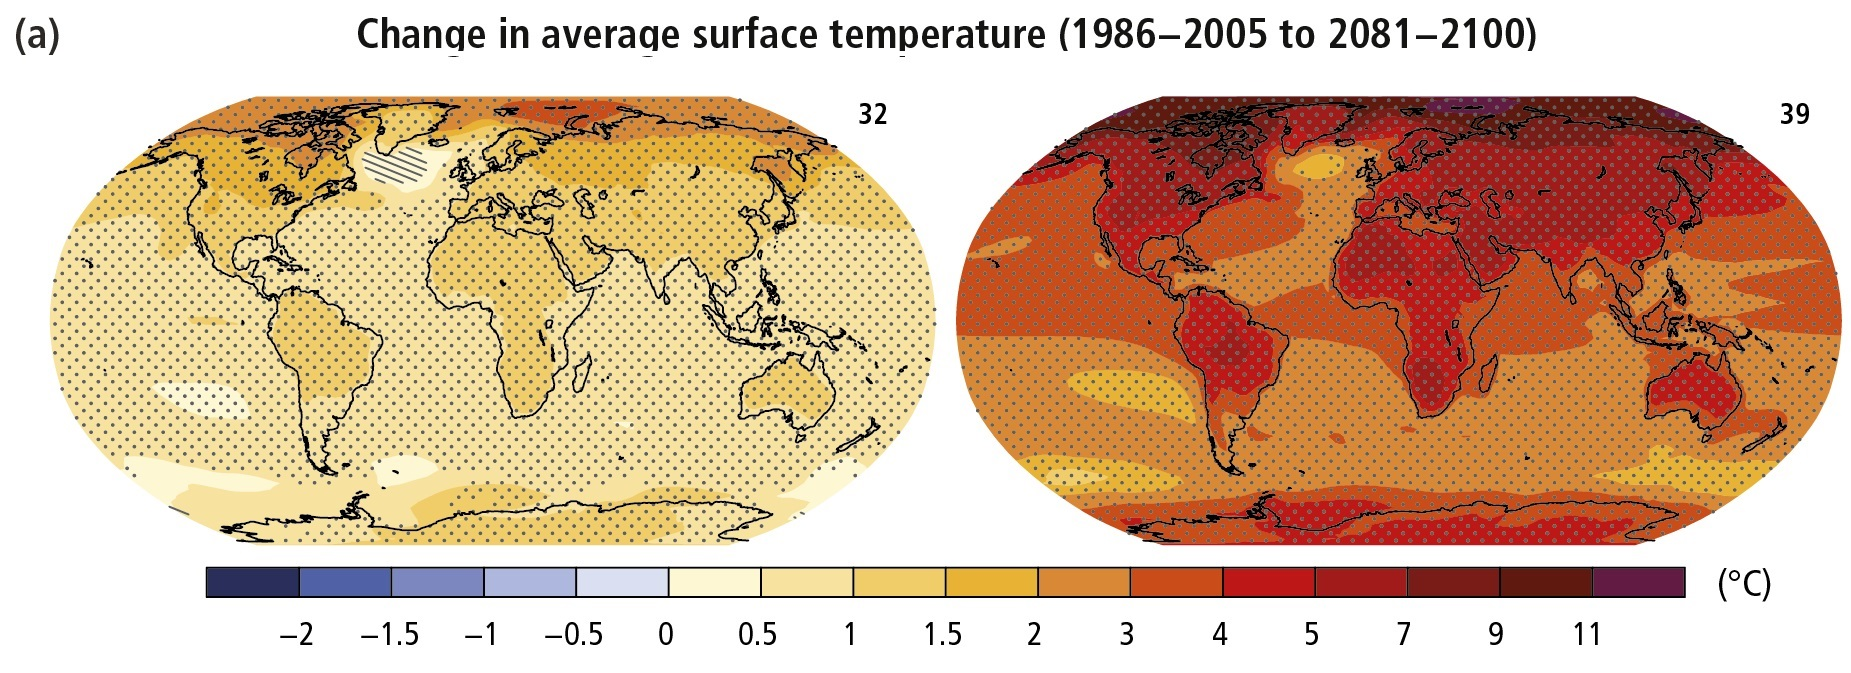
\includegraphics[scale=1.]{imagens/Temp_IPCC}
	\caption{Variação na temperatura geral da superfície da Terra durante os anos de 1986-2005 para 2081-2100. Fonte: IPCC. }
	
	\label{fig:TempE}
\end{figure}
\FloatBarrier


Como apontado por \citeauthorandyear{weitemeyer2015integration}, o uso de energias renováveis na Europa tem aumentado, considerando as preocupações em relação as alterações climáticas. Como citado pelo autor, devido à facilidade imposta pelo ambiente, considerando um objetivo onde o uso da geração será prioritariamente por fontes renováveis, tem-se o uso da energia solar e eólica como pontos chaves para se alcançar esse objetivo. Como simulado e mostrado na figura~\ref{fig:Wind_sol}, o uso de energias renováveis se mostra promissor na simulação considerando a Alemanha como objeto de estudo, tendo apenas a geração estrita por meio de energia solar, distante do cenário de integração perfeita, onde $\alpha$=0 representa uma geração estritamente solar, e $\alpha$=1 representa uma geração estritamente eólica.

\FloatBarrier
\begin{figure}[htbp]
	\centering
	%scale redimensiona a figura.
	%1.5 = 150% do tamanho original
	%1 = 100% do tamanho original
	%0.20 = 20% do tamanho original
	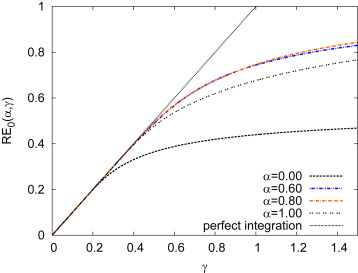
\includegraphics[scale=1.5]{imagens/wind_solar}
	\caption{Simulação do uso de energias renováveis na Alemanha, utilizando-se diferentes ponderações na divisão entre fontes de geração solar e eólica. Fonte:  \citeauthorandyear{weitemeyer2015integration} }
	
	\label{fig:Wind_sol}
\end{figure}
\FloatBarrier

Tendo em vista o problema causado por energias provenientes de fontes fósseis, o Brasil se concentrou na geração de energia elétrica de fontes renováveis principalmente hidráulicas, atingindo um índice de mais de 74\% de sua produção de acordo com \citeauthorandyear{wanderley2013perspectivas} e conforme visto na figura~\ref{fig:FonteEnergia}.

Devido a oscilações anuais dos índices de chuva, o racionamento de energia causado pelas épocas de estiagem, excitou a busca por novas fontes energéticas alternativas; tendo em vista que o Brasil é um país de clima predominantemente tropical, houve um crescente  desenvolvimento de pesquisas para a produção de energia solar fotovoltaica. 

\FloatBarrier
\begin{figure}[htbp]
	\centering
	%scale redimensiona a figura.
	%1.5 = 150% do tamanho original
	%1 = 100% do tamanho original
	%0.20 = 20% do tamanho original
	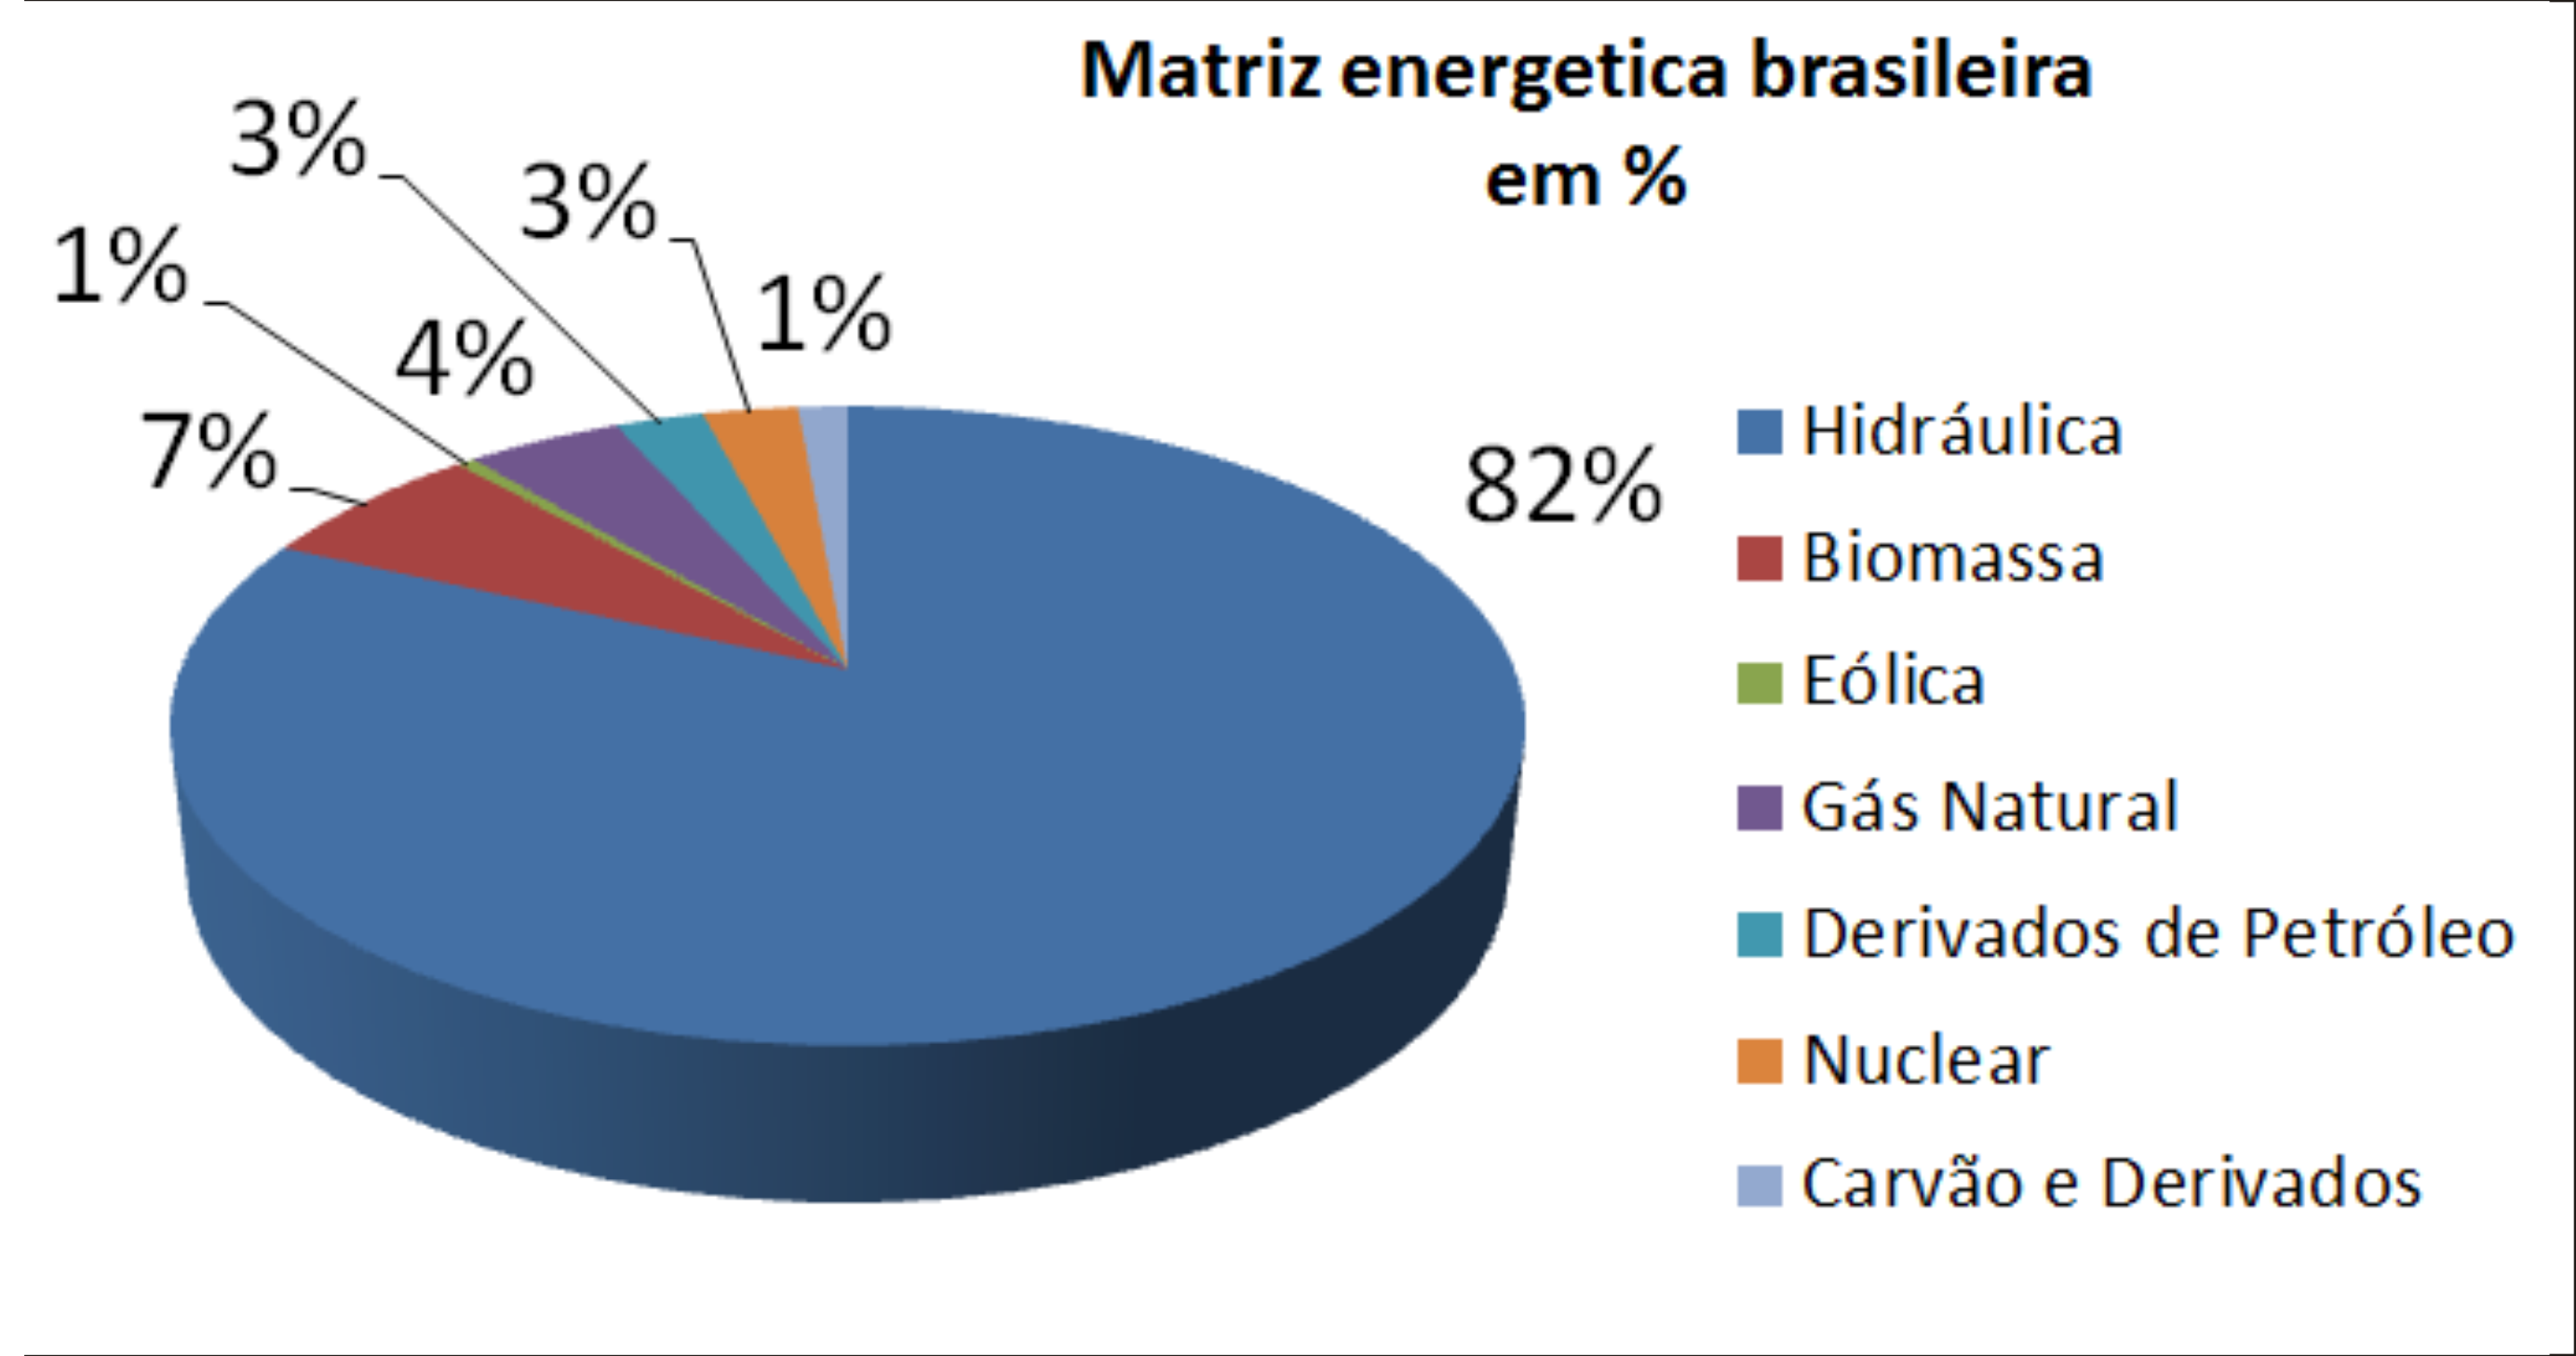
\includegraphics[scale=1]{imagens/FontesEnergia}
	\caption{Distribuição da matriz energética brasileira. Fonte:  \citeauthorandyear{wanderley2013perspectivas}. }
	
	\label{fig:FonteEnergia}
\end{figure}
\FloatBarrier

O grande impasse para produção de usinas solares é o alto valor de produção tendo em vista o rendimento dos painéis fotovoltaicos comparado  com as fontes de energias tradicionais. De acordo com \citeauthorandyear{ribeiro2017proposiccao}, para construir uma usina solar fotovoltaica com capacidade de produção de aproximadamente $4.000MWh$ ao ano, seria necessário um investimento de aproximadamente $R\$ 22.000.000,00$ ou seja, $7,30 R\$/Wp$; no artigo citado, foram taxados preços dos painéis, inversores, imposto de importação e taxas de produção. A solução para viabilizar a produção deste tipo de energia, seria o aumento de sua eficiência energética. Para alcançar este objetivo, foram efetuados diversos estudos, pesquisas e implementações de circuitos eletrônicos e projetos mecânicos.
 
Há trabalhos de pesquisa que visam obter o melhor aproveitamento da radiação solar criando sistemas mecânicos, \citeauthorandyear{WILLOUGHBY2018171},  enquanto alguns fazem comparações entre painéis com células obstruídas através de sombreamento \citeauthorandyear{BRESSAN20161181}, outros fazem a aplicação de diferentes aparatos para se obter energia perdida devido à difusão dos raios solares Lee et al. (2016), há trabalhos que propõem mensurar a perda de energia devido a poluição do ar em determinadas regiões \citeauthorandyear{li2017reduction}. Foram apresentados projetos que objetivam a melhora da potência entregue pelos painéis através no melhoramento da curva IxV (Corrente por tensão), foram apresentados projetos mostrando modos de melhoria desta curva, entre eles o algoritmo MPPT (Maximum Power Point Traking)\citeauthorandyear{WILLOUGHBY2018171}.  

\FloatBarrier
\begin{figure}[htbp]
	\centering
	%scale redimensiona a figura.
	%1.5 = 150% do tamanho original
	%1 = 100% do tamanho original
	%0.20 = 20% do tamanho original
	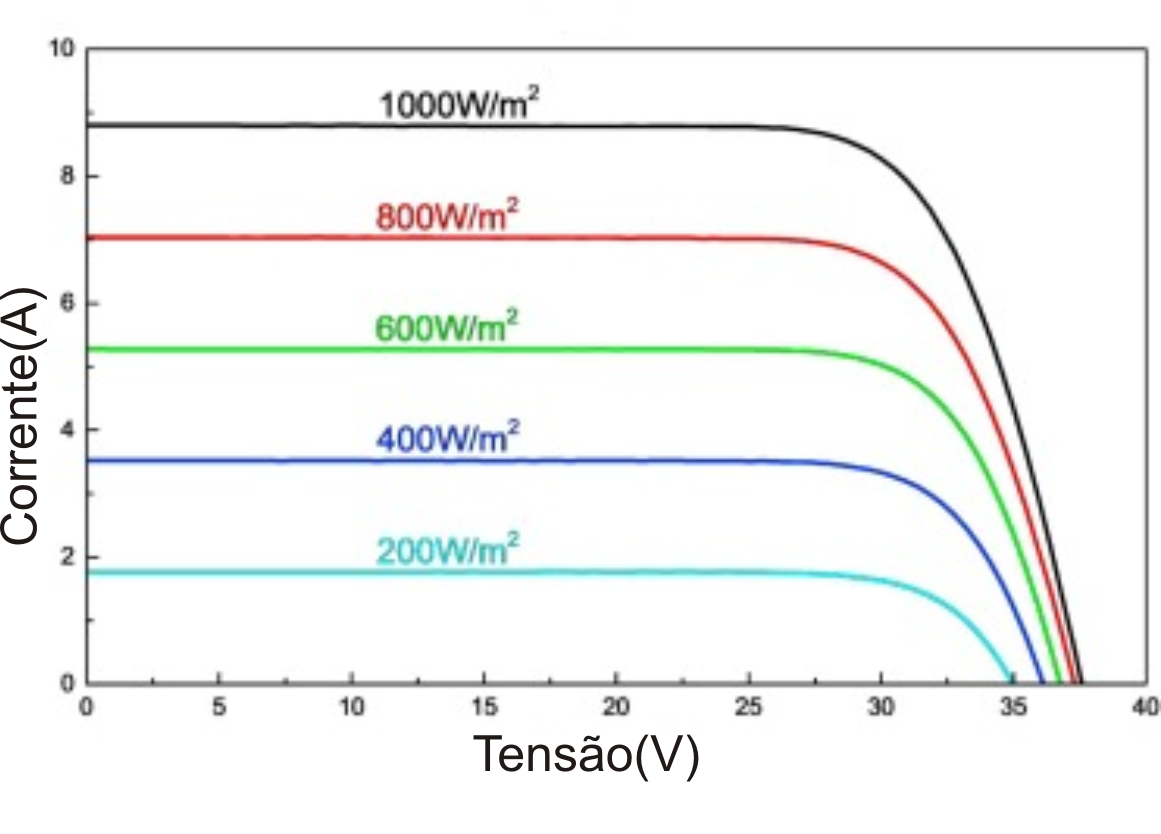
\includegraphics[scale=1.3]{imagens/IV_Gao}
	\caption{Curva IxV Característica de um painel fotovoltaico. Fonte:  \cite{GAO201852}.  }
	
	\label{fig:IVGao}
\end{figure}
\FloatBarrier

Para se obter um maior rendimento dos painéis fotovoltaicos, \citeauthorandyear{WILLOUGHBY2018171} apresentaram um projeto de um seguidor solar tendo por base um microcontrolador e motores de passo. A ideia proposta é a de que, durante o transcorrer do dia, o painel solar se modificaria sua inclinação de modo a estar sempre perpendicular a incidência dos raios solares, tendo assim uma potência de geração superior aos modelos convencionais com bases fixas.

Tomando uma abordagem diferente, porém com o mesmo intuito, Lee et al. (2016) publicaram \textit{Concentrator photovoltaic module architectures with capabilities for capture and conversion of full global solar radiation}. No artigo citado, foi apresentada a ideia de um concentrador de raios solares fazendo uso das células fotovoltaicas do tipo 3J (esférica) e 4J (plana). 

Foram propostas duas tecnologias de funcionamentos similares:

\begin{itemize}
	\item O primeiro concentrador é uma placa translúcida composto por bolhas que é colocada na parte de cima do painel com um distanciamento de 10 centímetros, essas bolhas tem como função captar os raios solares difusos e concentrar sobre células fotovoltaicas do tipo 3J;
	\item O segundo concentrador tem o mesmo princípio de funcionamento, uma placa translúcida com bolhas de estrutura diferente da apresentada anteriormente é colocada na parte superior do painel com um distanciamento de aproximadamente 10 centímetros, mas ao invés de concentrar os raios solares em uma única célula 3J, a bolha capta a irradiância solar e distribui de maneira uniforme sobre uma célula do tipo 4J.
\end{itemize}

Os dois métodos exibem resultados de até 8\% mais eficiência energética em comparação aos painéis fotovoltaicos convencionais, isso dado ao aumento da concentração e direcionamento dos raios solares difusos sobre as células fotovoltaicas.

Foi colocado por\cite{li2017reduction}, um ponto negativo e preocupante a respeito da produção de energia fotovoltaica no território da China. Segundo o artigo publicado: \textit{Reduction of solar photovoltaic resources due to air pollution in China}, A China tem por pretensão a produção de 400 $GW$ de energia elétrica proveniente de painéis fotovoltaicos até 2023. Porém, o estudo realizado revela que atualmente a poluição aérea causada por aerossóis, diminui de forma significativa a produção de energia fotovoltaica, em destaque na região do centro, leste e nordeste no país, locais de maior concentração de indústrias, índice de poluição e necessidade de energia elétrica. Índices mostram uma perda de 35\% da energia produzida e 1,5 $kWh/m^2$ da irradiância solar em todo território descrito, as nuvens causam grande influência sobre a irradiância solar que atinge o solo daquela região, porém com o agravante, as perdas aumentaram significativamente.

Assim como descrito anteriormente, painéis fotovoltaicos possuem diversas características favoráveis à geração de energia por meios sustentáveis e limpos. Entretanto, como aponta \citeauthorandyear{BRESSAN20161181}, arranjos fotovoltaicos estão extremamente sujeitos a meios externos que podem afetar sua geração, como sujeira, ou sombreamento, fatores os quais causam um rápido aquecimento das células fotovoltaicas. Existem maneiras de amenizar esse efeitos, como o uso de diodos \textit{bypass}, entretanto o uso dessas técnicas não anulam esse efeitos por completo. Como mostrado na Figura~\ref{fig:Temp}, é possível observar a variação da temperatura, alterando consequentemente o funcionamento do painel fotovoltaico.

\FloatBarrier
\begin{figure}[htbp]
	\centering
	%scale redimensiona a figura.
	%1.5 = 150% do tamanho original
	%1 = 100% do tamanho original
	%0.20 = 20% do tamanho original
	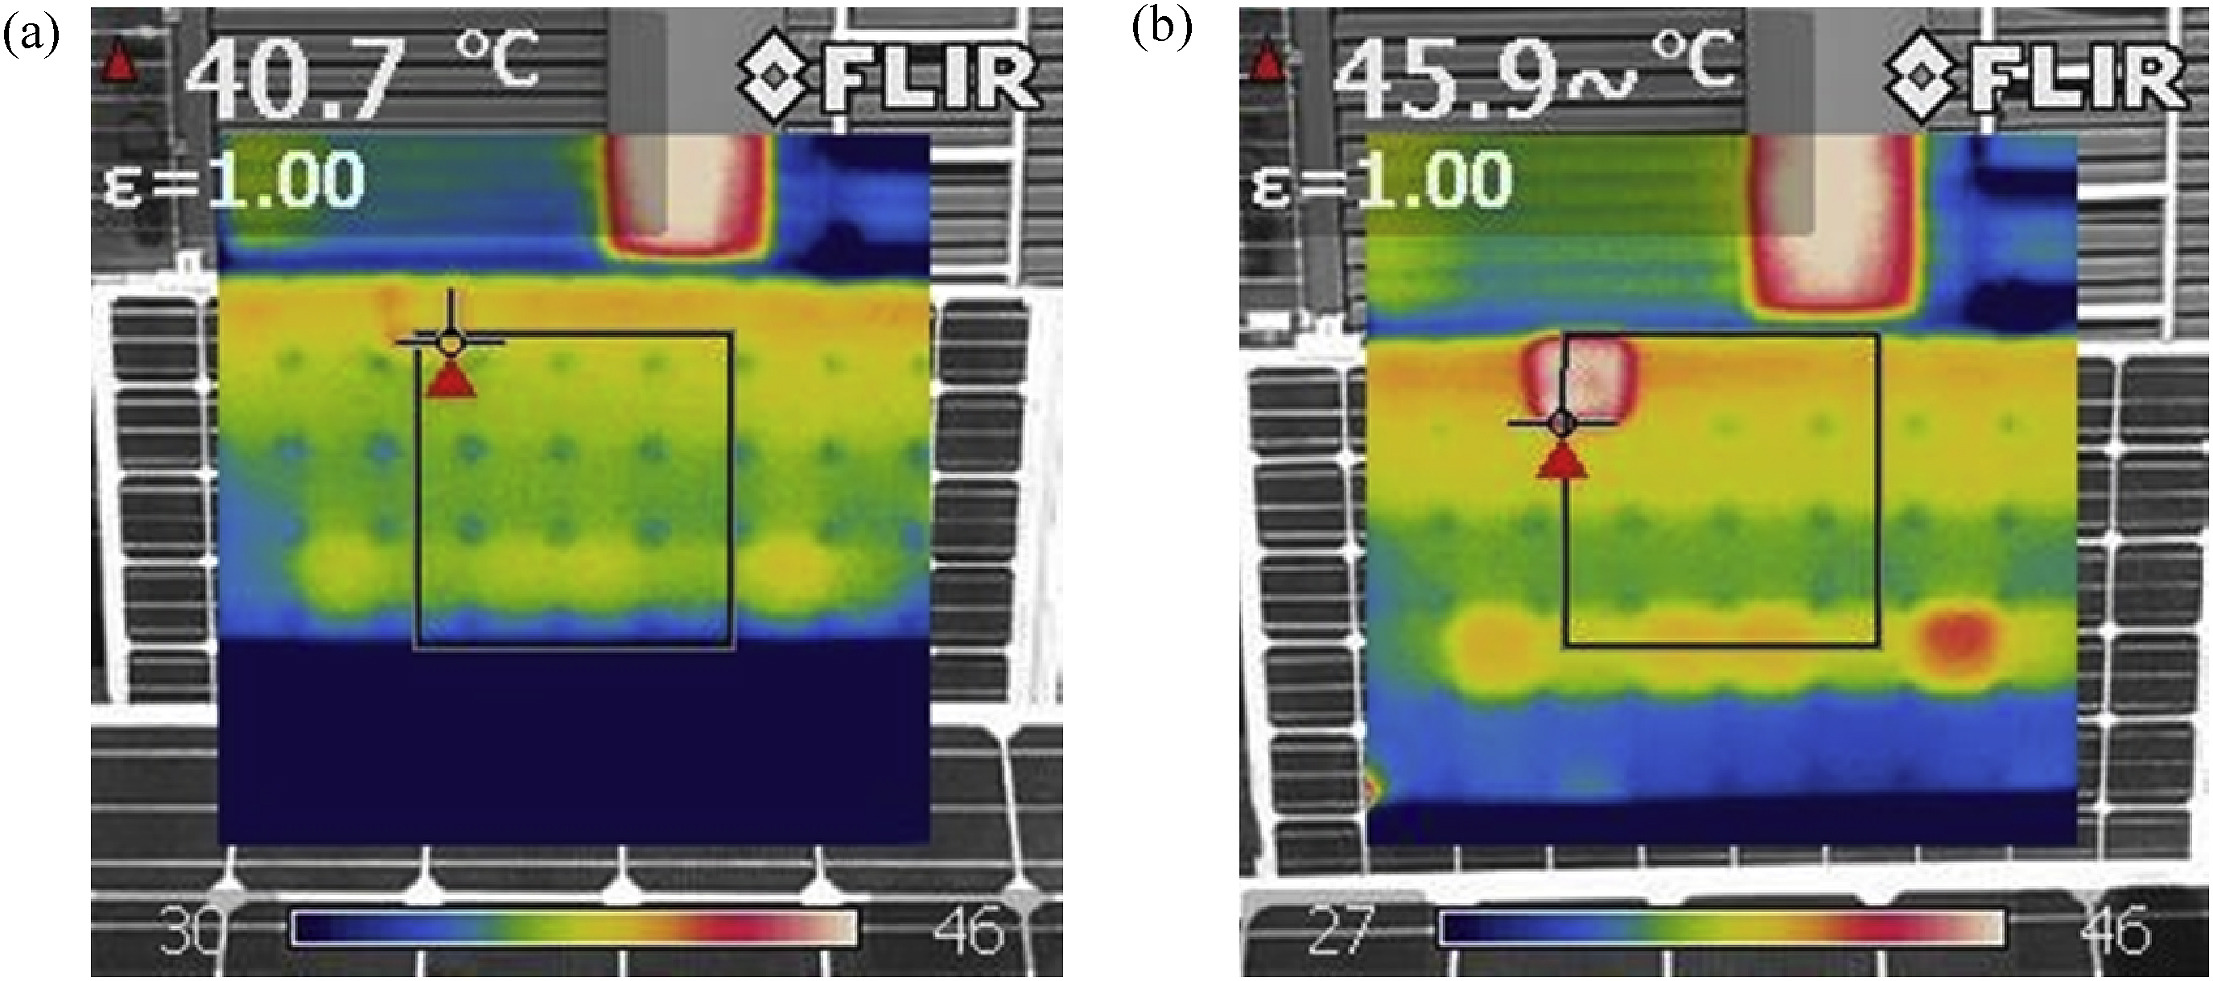
\includegraphics[scale=1.3]{imagens/Temp_BRESSAN}
	\caption{Variação na temperatura de células fotovoltaicas em um arranjo em curto-circuito. Fonte:  \citeauthorandyear{BRESSAN20161181} }
	
	\label{fig:Temp}
\end{figure}
\FloatBarrier

Como apontado anteriormente , há grande importância e interesse no uso da curva I-V de sistemas fotovoltaicos, para gerenciamento, funcionamento, e verificação de erros, assim como descreve \citeauthorandyear{SCHILL2015259} no \textit{Fraunhofer Institute for Solar Energy Systems ISE}, faz-se o uso da curva I-V para verificação da performance dos arranjos fotovoltaicos durantes teste em ambientes abertos para verificação da durabilidade de materiais para o uso em sistemas fotovoltaicos. De acordo com os autores, é verificado e monitorado a curva a cada 10 minutos. O uso da curva I-V permitiu a conclusão em teste onde os painéis foram sujos, durante o teste foi verificada uma diminuição de até 20\% dos valores iniciais de eficiência, sendo possível observar a diferença entre as curvas de placas limpas e placas sobre grande influência de poeira como visto na Figura~\ref{fig:CurvaIVNeve}.

\FloatBarrier
\begin{figure}[!htbp]
	\centering
	%scale redimensiona a figura.
	%1.5 = 150% do tamanho original
	%1 = 100% do tamanho original
	%0.20 = 20% do tamanho original
	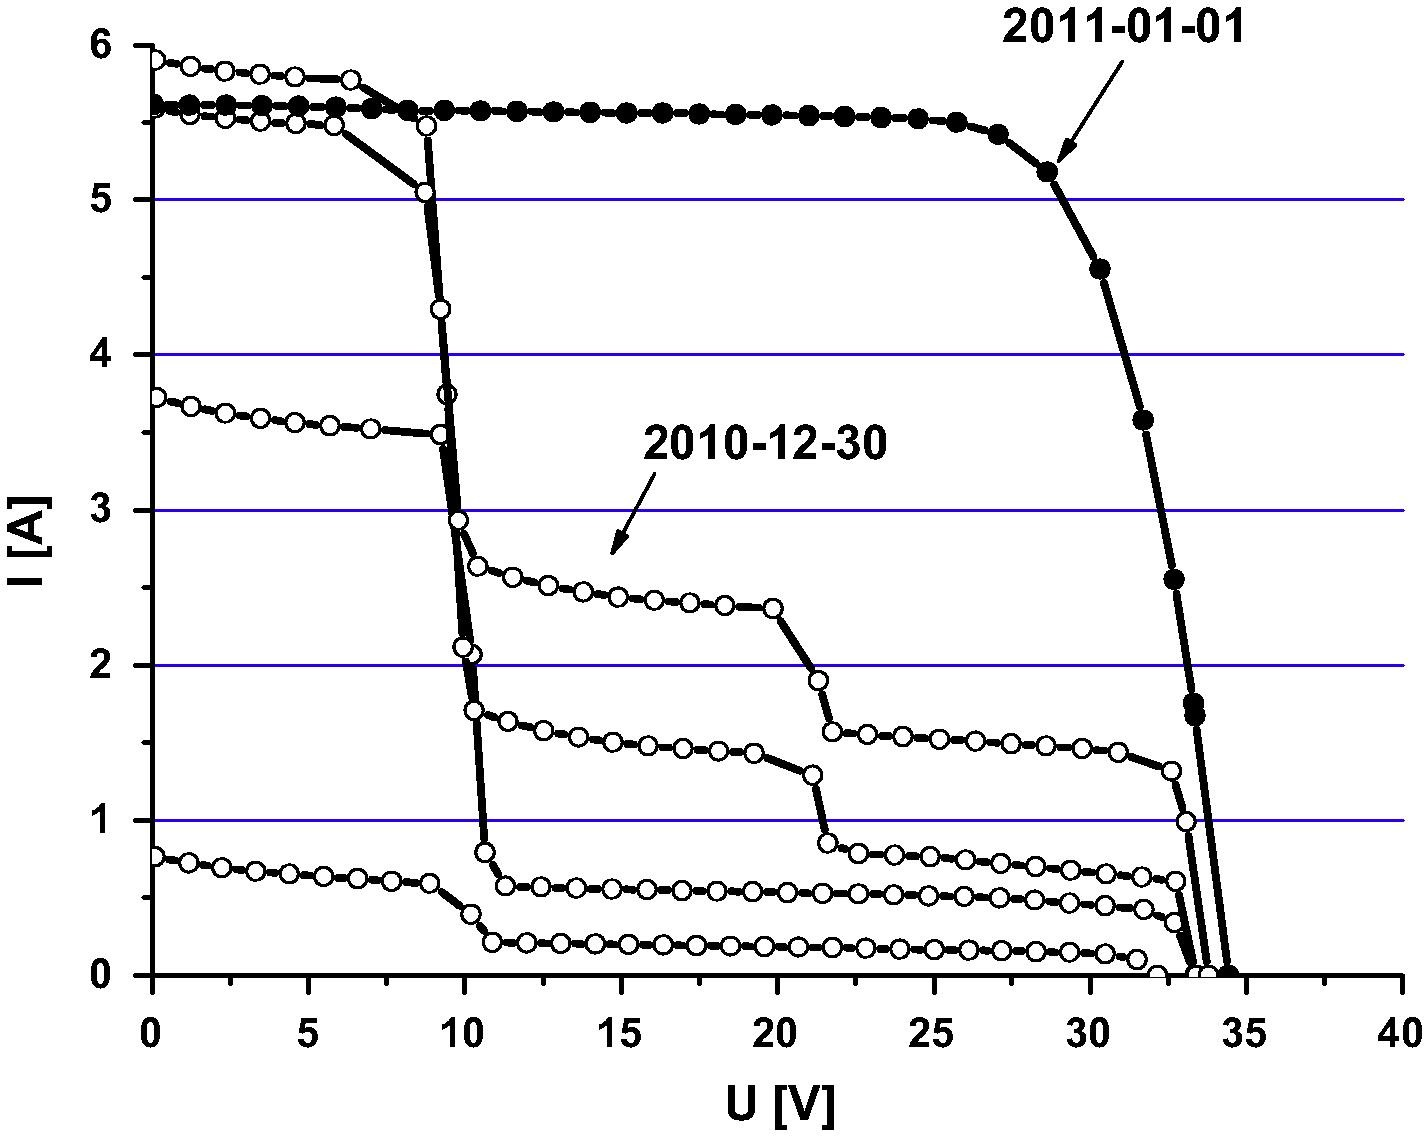
\includegraphics[scale=1.5]{imagens/IxV_schill}
	\caption{Curva característica I-V de painéis fotovoltaicos sobre influência de neve, a qual foi removida no dia 01/01. Fonte: \citeauthorandyear{SCHILL2015259}. }

	\label{fig:CurvaIVNeve}
\end{figure}
\FloatBarrier

Assim como analisado por \citeauthorandyear{martin2017temperature} , a temperatura do painel fotovoltaico possui influência sobre a geração, e respectiva curva I-V do painel em análise. É possível observar esse efeito na Figura~\ref{fig:IVTemp}.

\FloatBarrier
\begin{figure}[!htbp]
	\centering
	%scale redimensiona a figura.
	%1.5 = 150% do tamanho original
	%1 = 100% do tamanho original
	%0.20 = 20% do tamanho original
	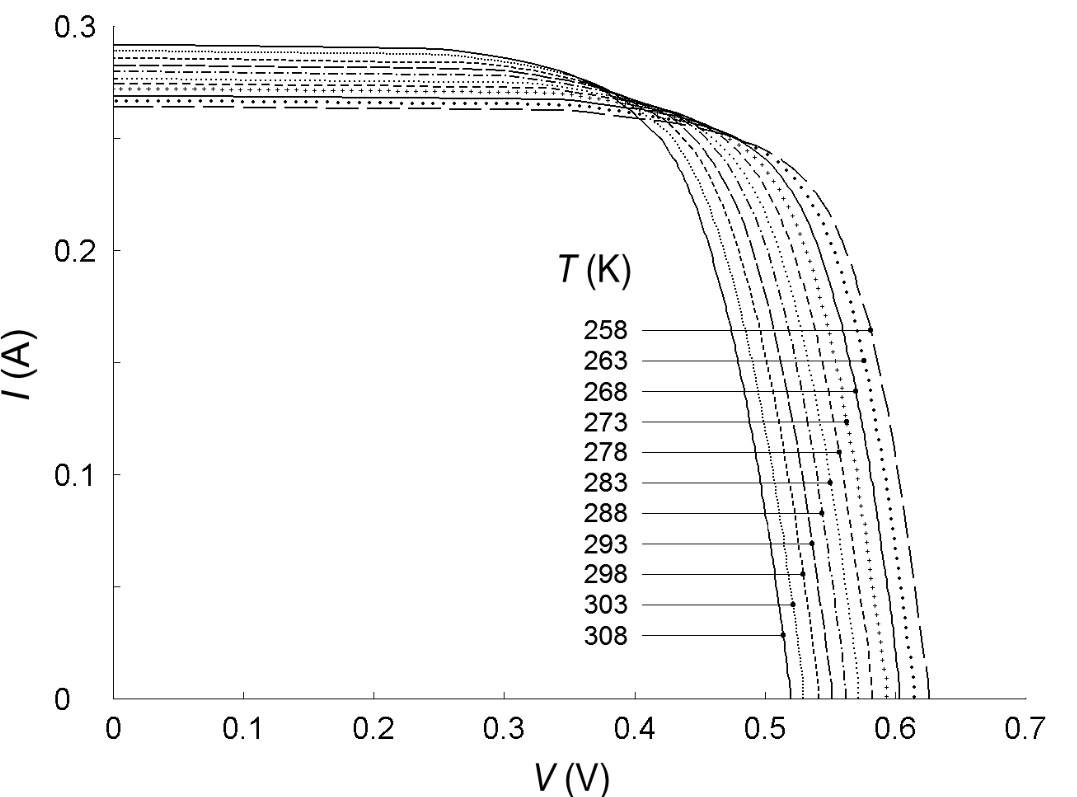
\includegraphics[scale=0.3]{imagens/IxV_Temp}
	\caption{Curva característica I-V de painéis fotovoltaicos sobre diferentes temperaturas. Fonte: \citeauthorandyear{martin2017temperature}. }
	
	\label{fig:IVTemp}
\end{figure}
\FloatBarrier

Assim como aponta \citeauthorandyear{SCHILL2015259}, o elemento central para a geração da curva I-V é a carga eletrônica, o qual tem como principal função simular diferentes cargas para o painel fotovoltaico, de maneira a permitir verificar seu comportamento, como foi descrito também por \citeauthorandyear{aliaga2016experimental}, na criação de sistemas que possam garantir a máxima potência global de um arranjo fotovoltaico. Um sistema de carga eletrônica com MOSFET, como mostrado na figura~\ref{fig:CargaELE} permite a rápida variação de carga sobre o painel fotovoltaico de maneira a possibilitar a construção da curva I-V característica do painel em determinado instante, desta maneira diminuir a diferença de geração devido a meios externos como nuvens ou variações climáticas, \cite{WILLOUGHBY2018171}.%(WILLOUGHBY; OSINOWO, 2018).

\FloatBarrier
\begin{figure}[!htbp]
	\centering
	%scale redimensiona a figura.
	%1.5 = 150% do tamanho original
	%1 = 100% do tamanho original
	%0.20 = 20% do tamanho original
	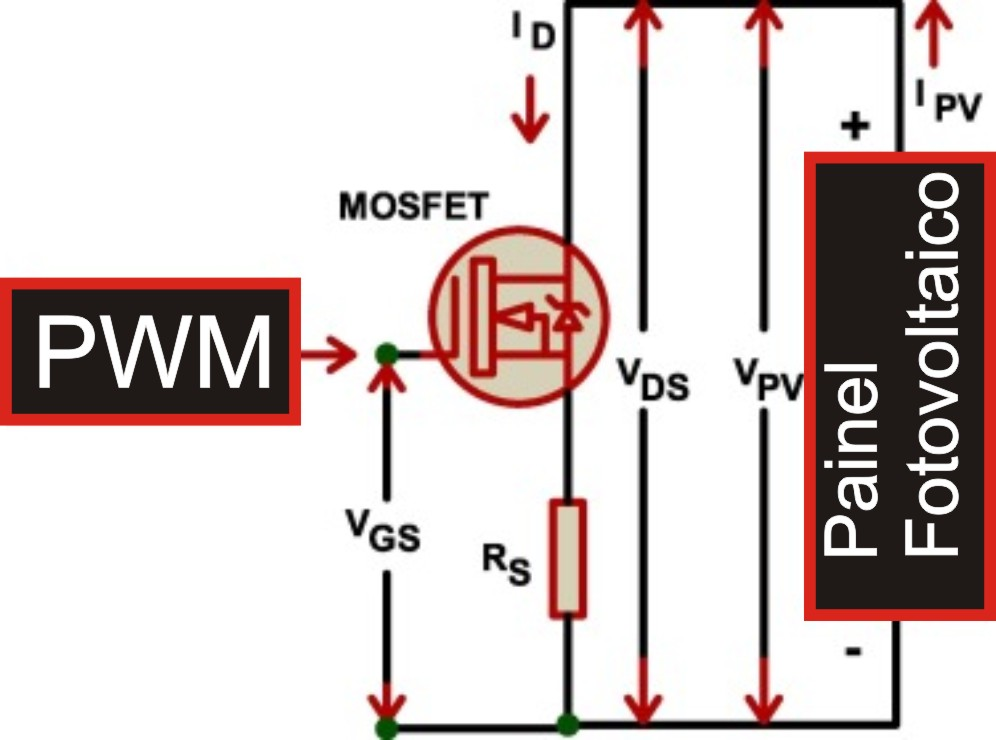
\includegraphics[scale=1]{imagens/MOSFET_LOAD}
	\caption{Uso de MOSFET como carga eletrônica para uso em painéis fotovoltaicos. Fonte: \citeauthorandyear{WILLOUGHBY2018171}. }
	
	\label{fig:CargaELE}
\end{figure}
\FloatBarrier

%\cite




Este é um exemplo de como usar tabelas. Referência cruzada: Tabela~\ref{tab:exemplo}

\FloatBarrier
\begin{table}[!htbp]
\centering
\caption{Exemplo de tabela de 2 colunas}
	\begin{tabular}{ c | c }
		\hline
		\textbf{Coluna 1} & \textbf{Coluna 2} \\ \hline
		Dado 1a           & Dado 1b           \\ \hline
		Dado 2a           & Dado 2b           \\ \hline
		Dado 3a           & Dado 3b           \\ \hline
		Dado 4a           & Dado 4b           \\ \hline
	\end{tabular}
	\\ \vspace{0.2cm}
	\textbf{Fonte:} Elaborada pelo autor
	\label{tab:exemplo}
\end{table}
\FloatBarrier


Este é um exemplo de como usar quadros. Referência cruzada: Quadro~\ref{qua:exemplo}

\FloatBarrier
\begin{quadro}[!htbp]
	\centering
	\caption{Exemplo de quadro}
	\includegraphics[scale=.7]{imagens/exemploQuadro}
	\\\textbf{Fonte:} Elaborada pelo autor
	\label{qua:exemplo}
\end{quadro}
\FloatBarrier


Este é um exemplo de como usar equações. Referência cruzada: Equação~\ref{eq:exemplo}

\begin{equation}
\sum_{i=1}^{n} = \frac{n(n+1)}{2}
\label{eq:exemplo}
\end{equation}


Exemplo de inserção de lista de código fonte (\textbf{\textcolor{red}{não use acentos no código!}}):

\lstinputlisting[language=Java]{fontes/ClasseExemplo.java} 



Este é um exemplo de como inserir texto sem formatação (ambiente verbatim):

\begin{verbatim}
	Texto sem formatação, como espaçamento igual.
\end{verbatim}


Exemplo de lista de itens:

\begin{itemize}
	\item \textbf{Item 1:} texto...;
	\item \textbf{Item 2:} texto...;
    \begin{itemize}
            \item \textbf{Subitem:} texto...;
            \item \textbf{Subitem:} texto...;
            \item \textbf{Subitem:} texto...;
        \end{itemize}
	\item \textbf{Item 3:} texto...;
	\item \textbf{Item n:} texto....
\end{itemize}


Exemplo de lista numerada:

\begin{enumerate}
	\item \textbf{Item:} texto...;
	\item \textbf{Item:} texto...;
    \begin{enumerate}
        \item \textbf{Subitem:} texto...;
        \item \textbf{Subitem:} texto...;
        \item \textbf{Subitem:} texto...;
    \end{enumerate}
	\item \textbf{Item:} texto...;
	\item \textbf{Item:} texto....
\end{enumerate}


Exemplos de comandos para texto e referências:

\begin{itemize}
	\item Para iniciar um novo parágrafo, basta deixar uma linha em branco no código fonte;
	\item Não force o compilador a pular mais de uma linha, pois terá influência negativa na composição do documento;
	\item Sempre deixe o \LaTeX\ realizar a formatação de parágrafos e posicionamento de elementos;
	\item Utilização de aspas simples (abertura \verb|`|, fechamento \verb|'|): `Texto entre aspas simples';
	\item Utilização de aspas duplas (abertura \verb|``|, fechamento \verb|''|): ``Texto entre aspas duplas'';
	\item Negrito (comando \verb|\textbf|): \textbf{texto em negrito};
	\item Itálico (comando \verb|\textit|): \textit{texto em itálico};
	\item Sublinhado (comando \verb|\underline|): \underline{texto sublinhado};
	\item Negrito e itálico (usar comandos juntos): \textbf{\textit{texto em negrito e itálico}};
	\item Alterar cor do texto (comando \verb|\textcolor{cor}{texto}|):
	\begin{itemize}
		\item Exemplo \verb|\textcolor{red}{texto}|: \textcolor{red}{texto vermelho};
		\item Exemplo \verb|\textcolor[RGB]{255, 102, 0}|: \textcolor[RGB]{255, 102, 0}{texto laranja};
		\item Exemplo \verb|\textcolor[HTML]{006AD7}|: \textcolor[HTML]{006AD7}{texto azul};
	\end{itemize}
	\item Ambiente matemático inline (comando \verb|$ expressão $|): $s = x^2-2x +1$;
	\item Referência normal (comando \verb|\cite|):
	\begin{itemize}
		\item \cite{Agaisse1995};
		\item \cite{Abedi2014};
		\item \cite{BtNomenclature2016};
	\end{itemize}
	\item Referência normal com mais de uma obra (comando \verb|\cite|):
	\begin{itemize}
		\item \cite{Agaisse1995, Abedi2014};
		\item \cite{Nelson2014, BtNomenclature2016, AgapitoTenfen2014};
	\end{itemize}
	\item Referência nome e ano (comando \verb|\citeauthorandyear|):
	\begin{itemize}
		\item %\citeauthorandyear{Agaisse1995};
		\item %\citeauthorandyear{Abedi2014};
		\item %\citeauthorandyear{BtNomenclature2016};
	\end{itemize}
\end{itemize}


Exemplo 1 de referência direta:

\begin{citacao}
	Os 20 aminoácidos usualmente encontrados como resíduos em proteínas contém um grupo $\alpha$-carboxil, um grupo $\alpha$-amino e um grupo R distinto substituído no átomo de carbono $\alpha$. O átomo de carbono $\alpha$ de todos os aminoácidos, com exceção da glicina, é assimétrico e, portanto, os aminoácidos podem existir em pelo menos duas formas estereoisoméricas. Somente os estereoisômeros L, com uma configuração relacionada à configuração absoluta da molécula de referência L-gliceraldeído, são encontrados em proteínas \cite[p. 81]{Nelson2014}
\end{citacao}

Exemplo 2 de referência direta:

\begin{citacao}
	\textit{These various insecticidal proteins are synthesized during the stationary phase and accumulate in the mother cell as a crystal inclusion which can account for up to 25\% of the dry weight of the sporulated cells. The amount of crystal protein produced by a B. thuringiensis culture in laboratory conditions (about 0.5 mg of protein per ml) and the size of the crystals (24) indicate that each cell has to synthesize $10^6$ to $2 \times 10^6$ $\delta$-endotoxin molecules during the stationary phase to form a crystal} \cite[p. 1]{Agaisse1995}
\end{citacao}

Exemplo de nota de rodapé\footnote{Essa é uma nota de rodapé!}.

\chapter{Materiais e Métodos}
\label{cap:03}

Para a prototipagem do traçador I-V houve a necessidade de se seguir as seguintes etapas:
\begin{itemize}
	\item Integração entre os componentes do protótipo sendo eles:
	\begin{itemize} 
		\item Arduino;
		\item Carga eletrônica;
		\item Painel solar;
		\item Sensor ADS1115;
		\item Cartão SD.
	\end{itemize}
	\item Teste de precisão na coleta de dados;
	\item Padronização e fixação do ambiente de testes;
	\item Teste do protótipo;
	\item Armazenamento da amostragem coletada;
	\item Análise e tratamento da amostra;
	\item Verificação e resolução de erros e/ou problemas.

\end{itemize}

\section{Arduino}
A plataforma Arduino, figura~\ref{fig:CircuitoDuino}, foi utilizada de maneira centralizar o controle de todos os periféricos necessários para a prototipagem. Foi utilizado as saídas PWM, Barramento I2C e SPI.

\FloatBarrier
\begin{figure}[!htbp]
	\centering
	%scale redimensiona a figura.
	%1.5 = 150% do tamanho original
	%1 = 100% do tamanho original
	%0.20 = 20% do tamanho original
	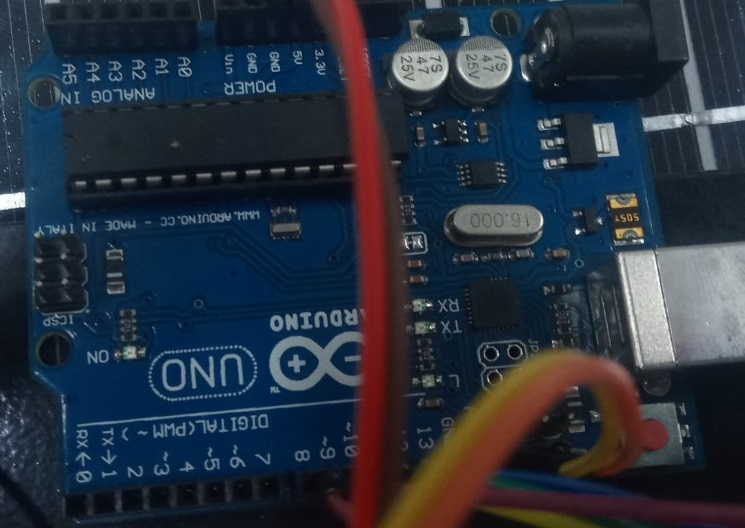
\includegraphics[scale=0.3]{imagens/ArduinoLigacoes.jpg}
	\caption{Arduino utilizado. Fonte: Elaborado pelo Autor. 	}
	\label{fig:CircuitoDuino}
\end{figure}
\FloatBarrier

\subsection{I2C e SPI}
As comunicações I2C e SPI, figura~\ref{fig:SPII2c}, permitiram o uso de ferramentas não disponíveis no hardware original do Arduino, como a utilização de um ADC de 16 bits ou do cartão SD para armazenamento dos dados, figura~\ref{fig:SDCard}.

\FloatBarrier
\begin{figure}[!htbp]
	\centering
	%scale redimensiona a figura.
	%1.5 = 150% do tamanho original
	%1 = 100% do tamanho original
	%0.20 = 20% do tamanho original
	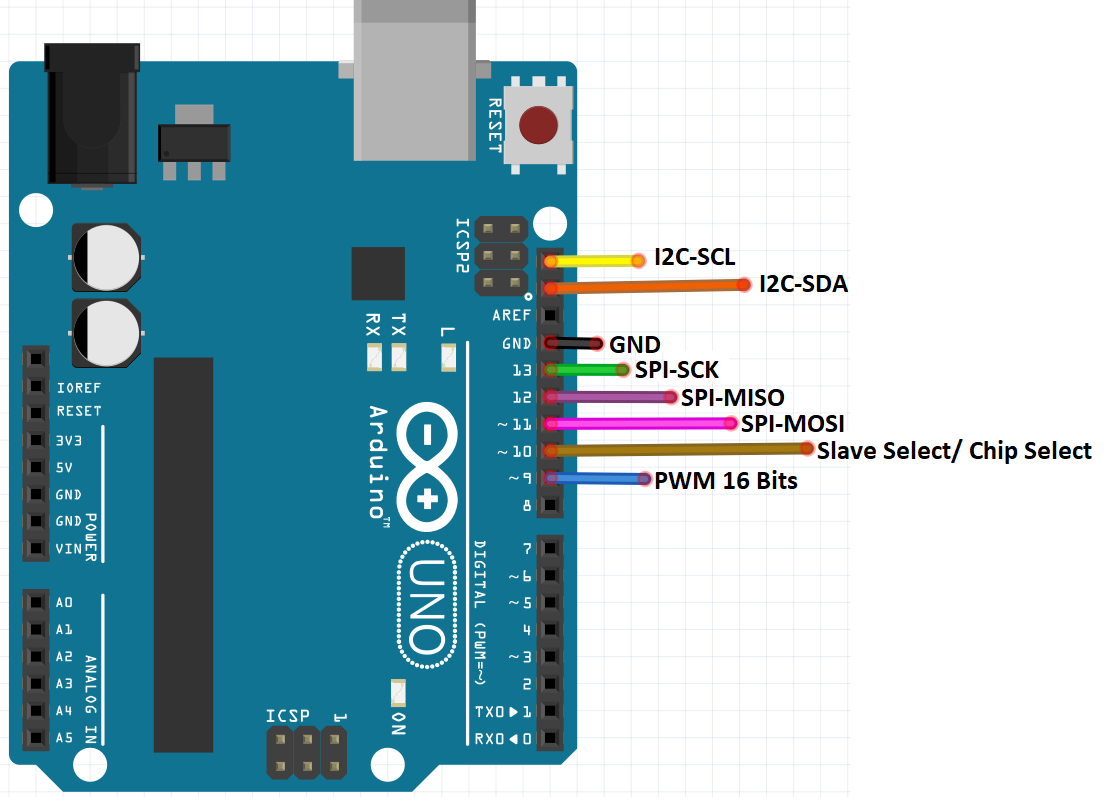
\includegraphics[scale=0.3]{imagens/ArduinoSPI_I2C.png}
	\caption{Ligações I2C e SPI do Arduino. Fonte: Elaborado pelo Autor. 	}
	\label{fig:SPII2c}
\end{figure}
\FloatBarrier

\FloatBarrier
\begin{figure}[!htbp]
	\centering
	%scale redimensiona a figura.
	%1.5 = 150% do tamanho original
	%1 = 100% do tamanho original
	%0.20 = 20% do tamanho original
	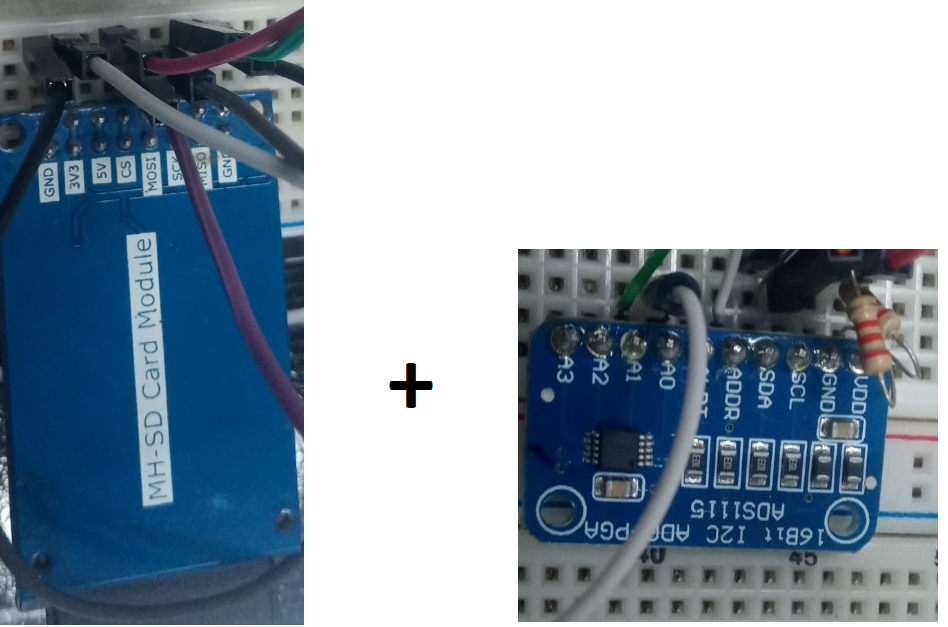
\includegraphics[scale=0.3]{imagens/SdcardADS.jpg}
	\caption{Dispositivos I2C e SPI utilizado pelo Arduino. Fonte: Elaborado pelo Autor. 	}
	\label{fig:SDCard}
\end{figure}
\FloatBarrier

\section{Carga Eletrônica}
A carga eletrônica, figura~\ref{fig:Carga}, permitiu a variação dos valores de corrente e tensão do painel, fator indispensável para a ação do traçador.

\FloatBarrier
\begin{figure}[!htbp]
	\centering
	%scale redimensiona a figura.
	%1.5 = 150% do tamanho original
	%1 = 100% do tamanho original
	%0.20 = 20% do tamanho original
	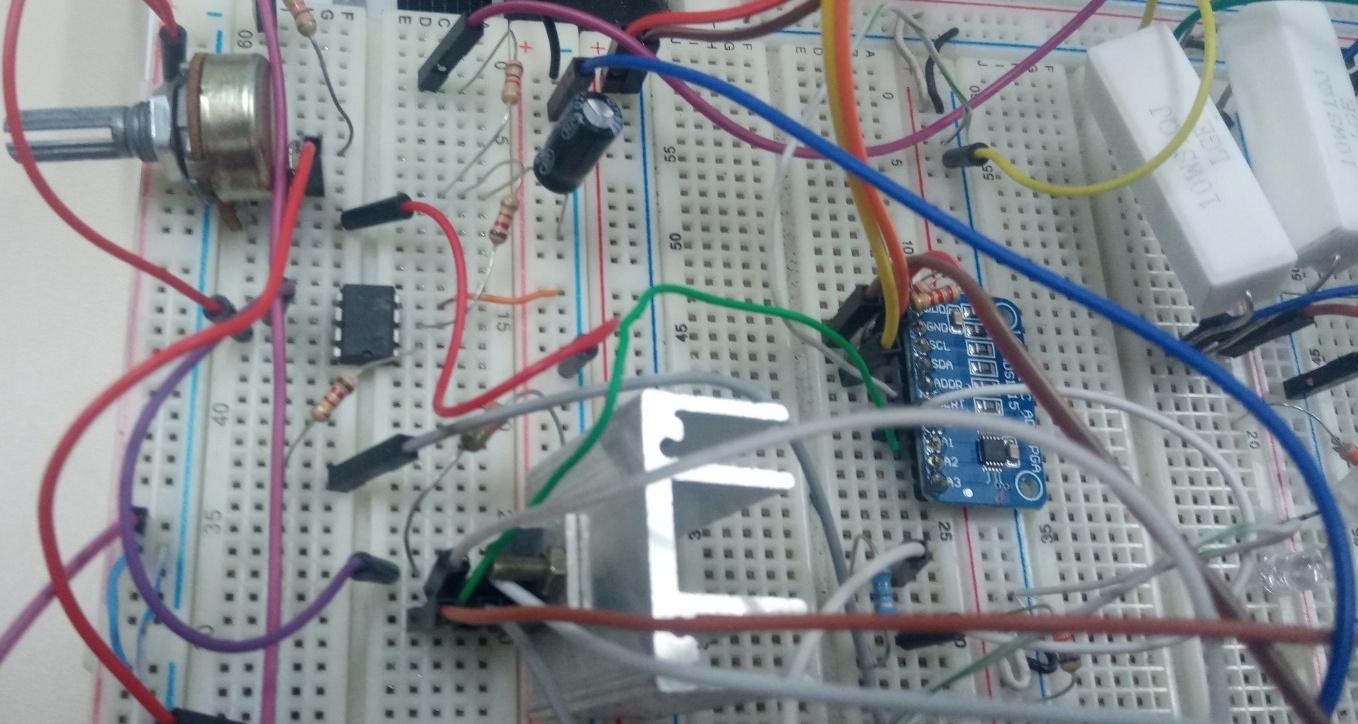
\includegraphics[scale=0.3]{imagens/CargaEletronica.png}
	\caption{Carga eletrônica. Fonte: Elaborado pelo Autor. 	}
	\label{fig:Carga}
\end{figure}
\FloatBarrier

\section{Lâmpada Halógena}
Houve o uso da lâmpada halógena de 500W, o qual simulou a luz solar, figura~\ref{fig:Lamp}, para permitir a realização dos experimentos em dias com pouca insolação.

\FloatBarrier
\begin{figure}[!htbp]
	\centering
	%scale redimensiona a figura.
	%1.5 = 150% do tamanho original
	%1 = 100% do tamanho original
	%0.20 = 20% do tamanho original
	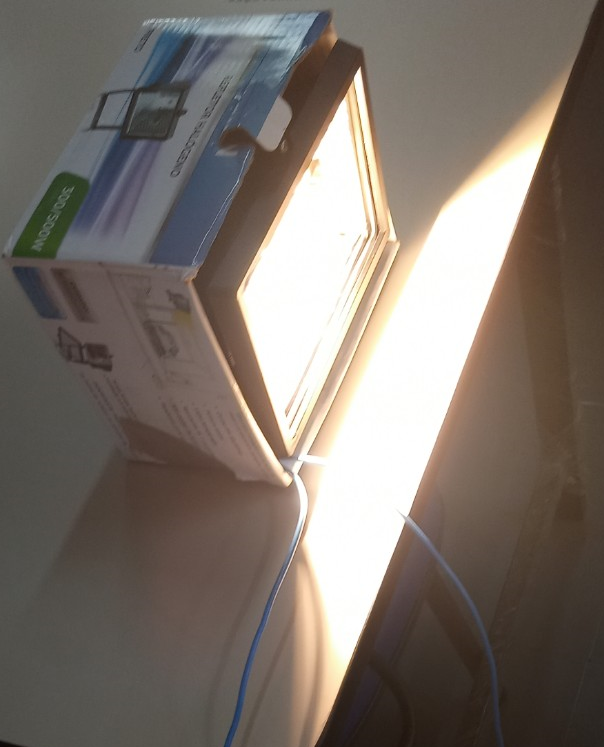
\includegraphics[scale=0.65]{imagens/Lamp.png}
	\caption{Lâmpada de 500W utilizada. Fonte: Elaborado pelo Autor. 	}
	\label{fig:Lamp}
\end{figure}
\FloatBarrier


\section{Circuito Completo}

Se observa na figura~\ref{fig:Circuito}, assim como no apêndice~\ref{Anx1}, como se assemelha o circuito eletrônico completo do traçador de curvas I-V.


\FloatBarrier
\begin{figure}[!htbp]
	\centering
	%scale redimensiona a figura.
	%1.5 = 150% do tamanho original
	%1 = 100% do tamanho original
	%0.20 = 20% do tamanho original
	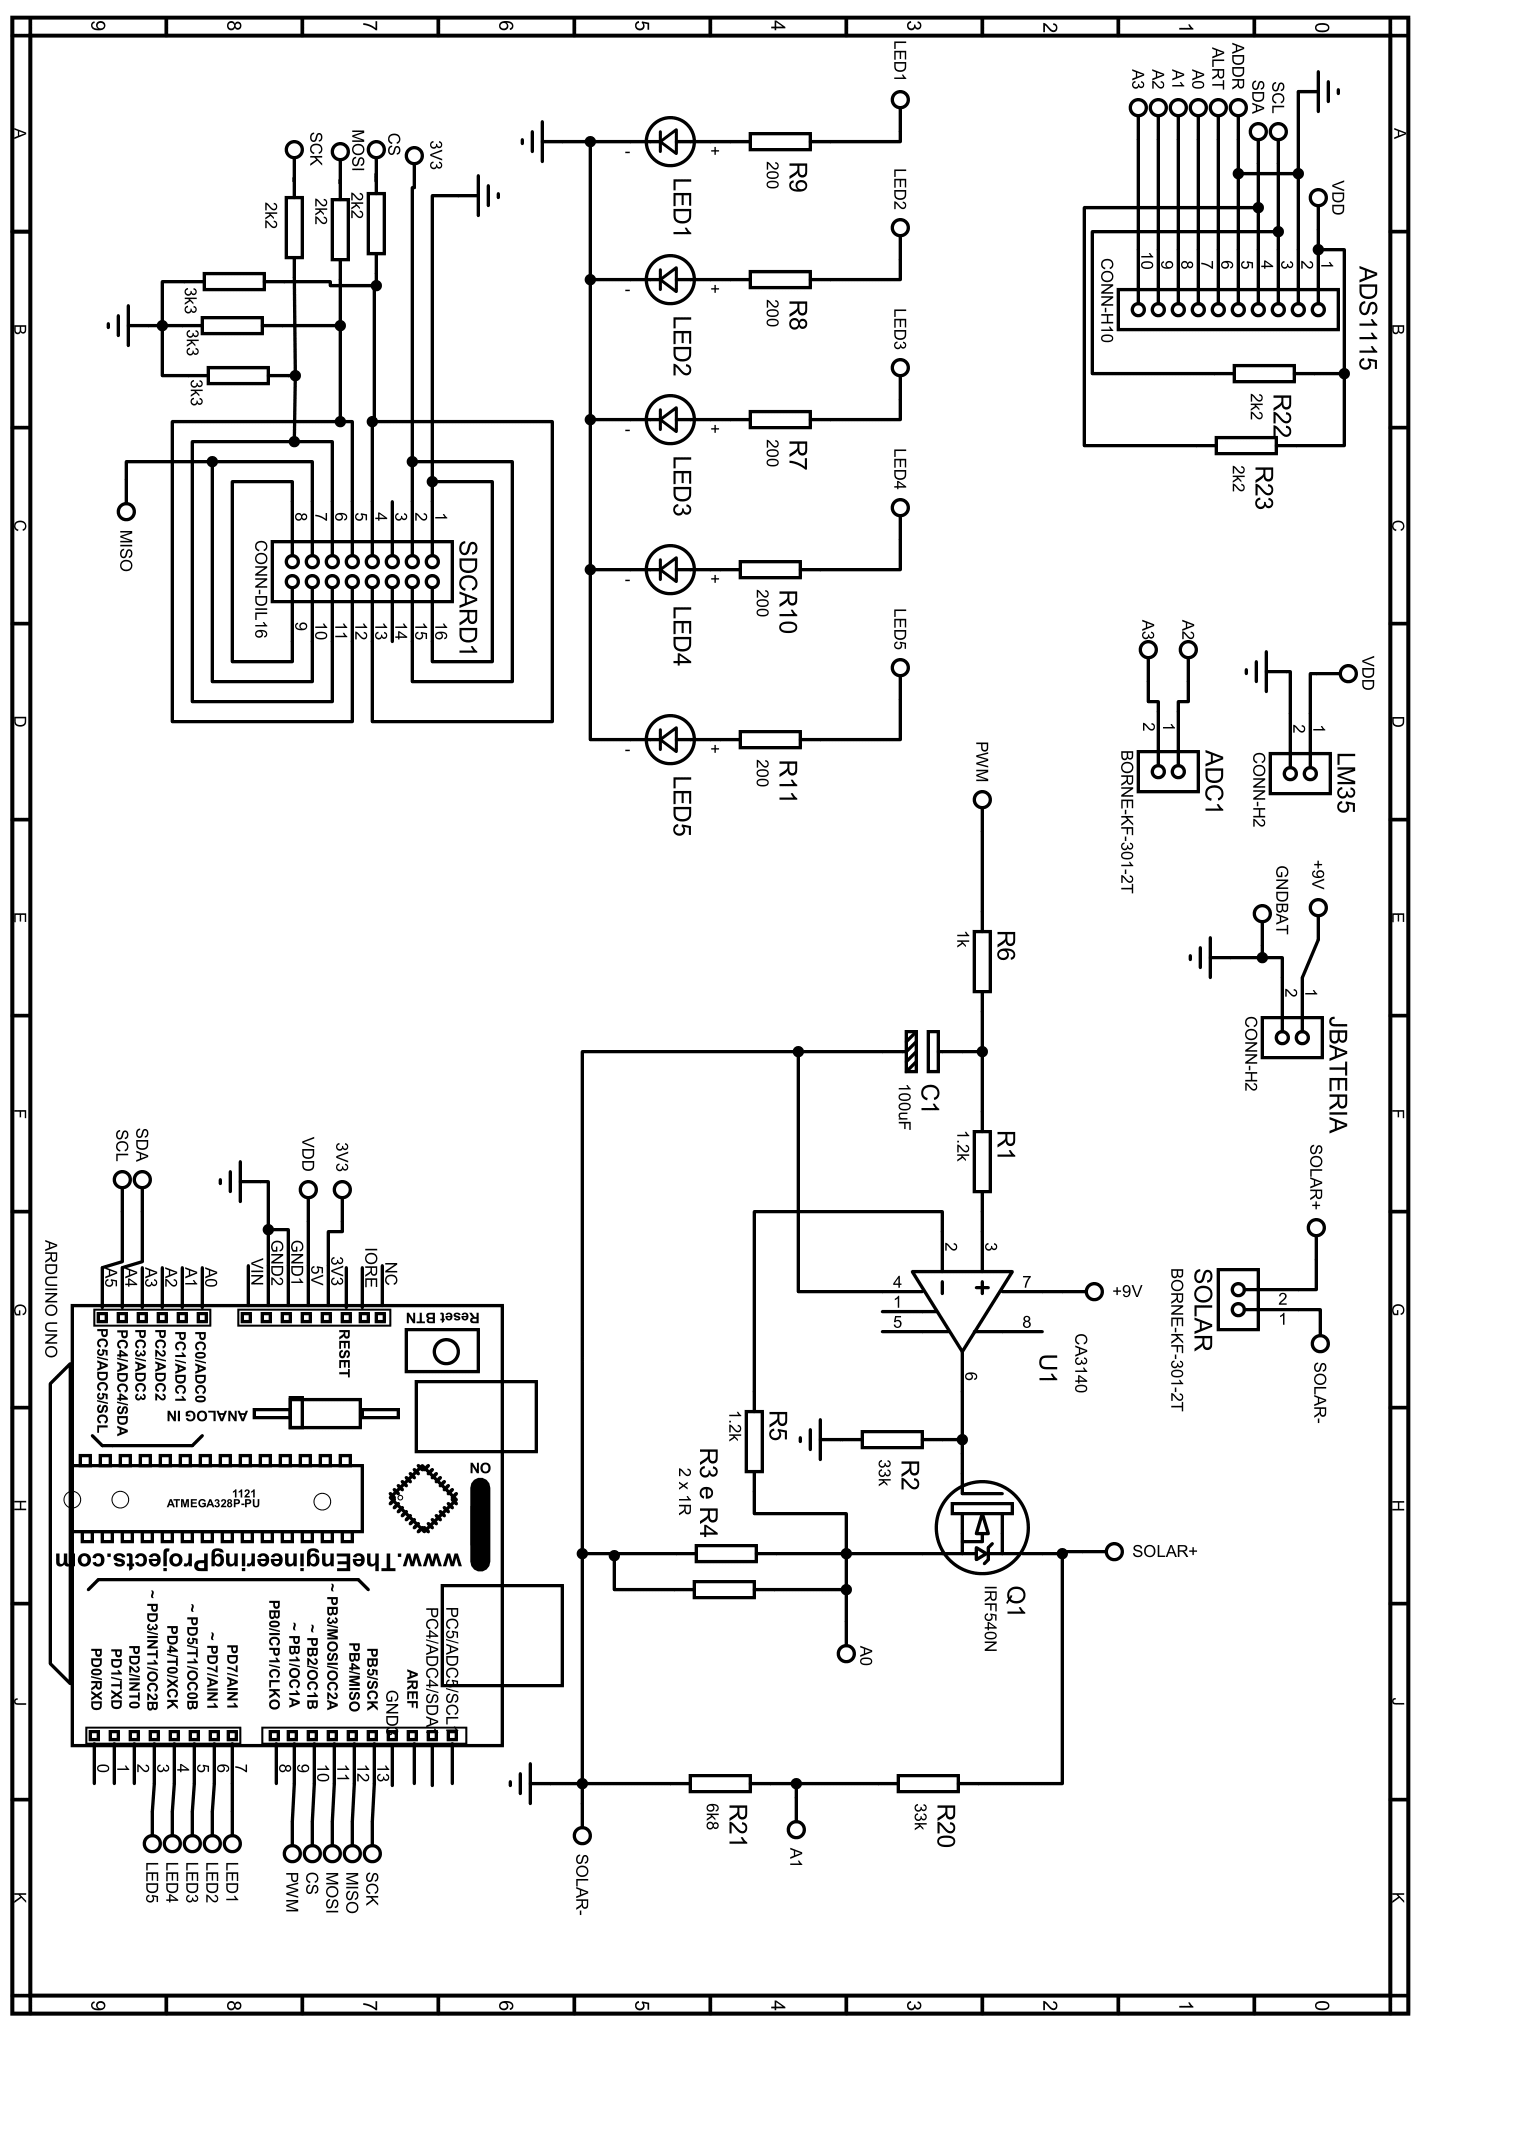
\includegraphics[scale=0.3]{PDFs/AllComponents-rotated-1.png}
	\caption{Circuito eletrônico completo. Fonte: Elaborado pelo Autor. 	}
	\label{fig:Circuito}
\end{figure}
\FloatBarrier

O circuito poder se dividido em:
\begin{enumerate}
	\item Conexões com o Arduino;
	\item Conexões Módulos;
	\item Carga Eletrônica;
	\item LEDs para sinalização.
\end{enumerate}

	
\subsection{Conexões com o Arduino}

A primeira parte do circuito,  figura~\ref{fig:CircuitoArduino}, as entradas e saídas disposta pelo Arduino e utilizadas para os acionamentos e sensoriamentos.

\begin{figure}[!htbp]
	\centering
	%scale redimensiona a figura.
	%1.5 = 150% do tamanho original
	%1 = 100% do tamanho original
	%0.20 = 20% do tamanho original
	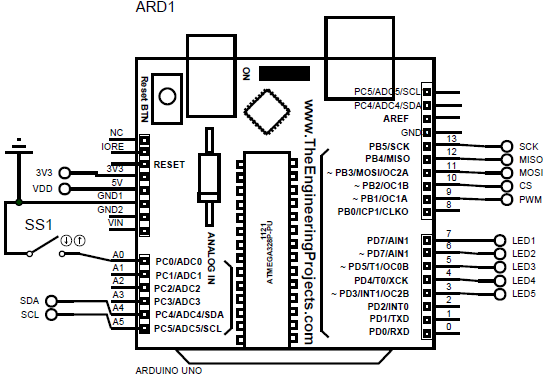
\includegraphics[scale=0.75]{imagens/CircuitoArduino.png}
	\caption{Circuito eletrônico, foco nos componentes mais próximos ao Arduino. Fonte: Elaborado pelo Autor utilizando a biblioteca \textit{Arduino Library for Proteus} disponível em \url{https://www.theengineeringprojects.com/2015/12/arduino-library-proteus-simulation.html}. 	}
	\label{fig:CircuitoArduino}
\end{figure}
\FloatBarrier

Na figura~\ref{fig:CircuitoArduino} se observa as conexões de alimentação dos módulos, os pinos das conexões de diferentes redes, sendo elas I2C e SPI. Há também os pinos conectados aos LEDs e ao botão que inicia o processo.

\subsection{Conexões Módulos}

A segunda parte do circuito,  figura~\ref{fig:CircuitoMod}, diz respeito aos conectores que serão utilizados para os módulos auxiliares para o processo da carga eletrônica.

\begin{figure}[!htbp]
	\centering
	%scale redimensiona a figura.
	%1.5 = 150% do tamanho original
	%1 = 100% do tamanho original
	%0.20 = 20% do tamanho original
	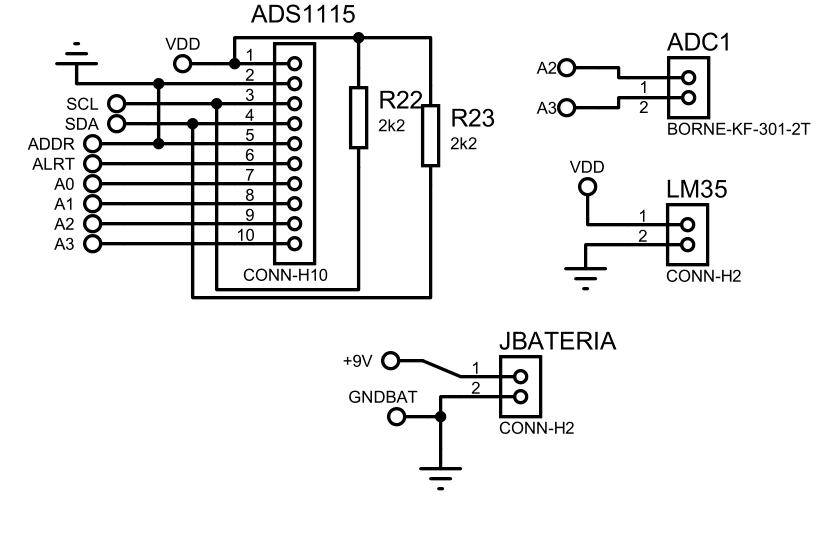
\includegraphics[scale=0.5]{imagens/CircuitoMod.png}
	\caption{Circuito eletrônico, foco nas conexões com o módulo. Fonte: Elaborado pelo Autor. 	}
	\label{fig:CircuitoMod}
\end{figure}
\FloatBarrier

Na figura~\ref{fig:CircuitoMod} se observa as conexões para os módulos, Cartão SD e ADS1115, além de conexões auxiliares para a o LM35, sensor de temperatura e para os sinais de entrada do módulo ADS1115.

\subsection{Carga Eletrônica}

A terceira parte do circuito,  figura~\ref{fig:CircuitoElet}, a carga eletrônica, principal circuito para o funcionamento do protótipo.

\begin{figure}[!htbp]
	\centering
	%scale redimensiona a figura.
	%1.5 = 150% do tamanho original
	%1 = 100% do tamanho original
	%0.20 = 20% do tamanho original
	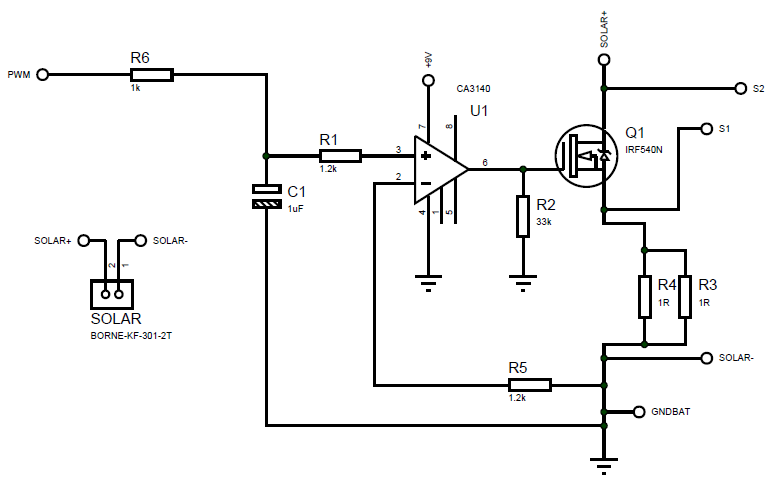
\includegraphics[scale=0.5]{imagens/CircuitoElet.png}
	\caption{Circuito eletrônico, foco na carga eletrônica. Fonte: Elaborado pelo Autor. 	}
	\label{fig:CircuitoElet}
\end{figure}
\FloatBarrier

Na figura~\ref{fig:CircuitoElet} se observa os componentes para o uso da carga eletrônica. Há também a presença dos conectores para os cabos provenientes do painel solar.

\subsection{Conjunto de LEDs}

A parte final do circuito,  figura~\ref{fig:CircuitoLED}, o conjunto de LEDs, \textit{Light-Emitting Diode}, Diodo Emissor de Luz, o qual tem como principal função garantir uma interface visual para o usuário, permitindo assim se encontrar durante o processo e erros ocorridos.

\begin{figure}[!htbp]
	\centering
	%scale redimensiona a figura.
	%1.5 = 150% do tamanho original
	%1 = 100% do tamanho original
	%0.20 = 20% do tamanho original
	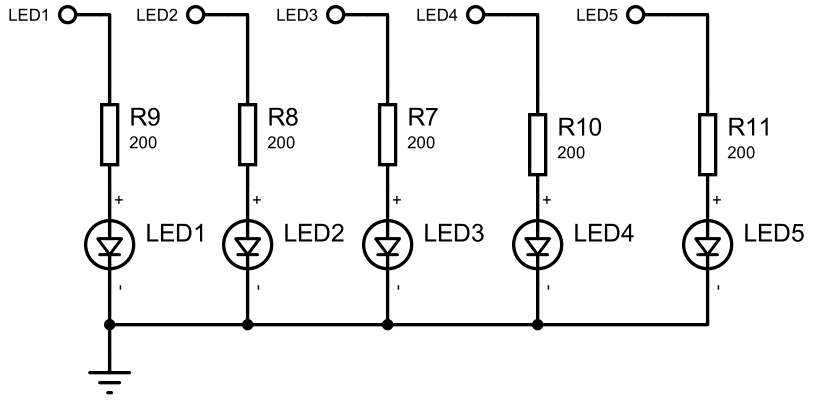
\includegraphics[scale=0.8]{imagens/CircuitoLED.png}
	\caption{Circuito eletrônico, foco no conjunto de LEDs. Fonte: Elaborado pelo Autor. 	}
	\label{fig:CircuitoLED}
\end{figure}
\FloatBarrier

Na figura~\ref{fig:CircuitoLED} se observa os cinco LEDs utilizados para o informativo ao usuário.

\section{Controle de Variáveis}
Durante os experimentos foram necessários atestar alguns aspectos, garantindo maior estabilidade no processo de aquisição de dados:
\begin{itemize}
\item Irradiância solar fixa;
\item Uso de sensores precisos.
\end{itemize}

Para garantir maior acuracidade e precisão na coleta de dados, foi realizado um teste com 30 diferentes valores a serem coletados pelo sensor utilizando ADS1115 e um multímetro de alta precisão. Ao se comparar os dados do multímetro e do ADS1115, nota-se os valores correspondentes do sensor em relação ao multímetro, como pode ser observado na figura~\ref{fig:Precisao}.

\FloatBarrier
\begin{figure}[!htbp]
	\centering
	%scale redimensiona a figura.
	%1.5 = 150% do tamanho original
	%1 = 100% do tamanho original
	%0.20 = 20% do tamanho original
	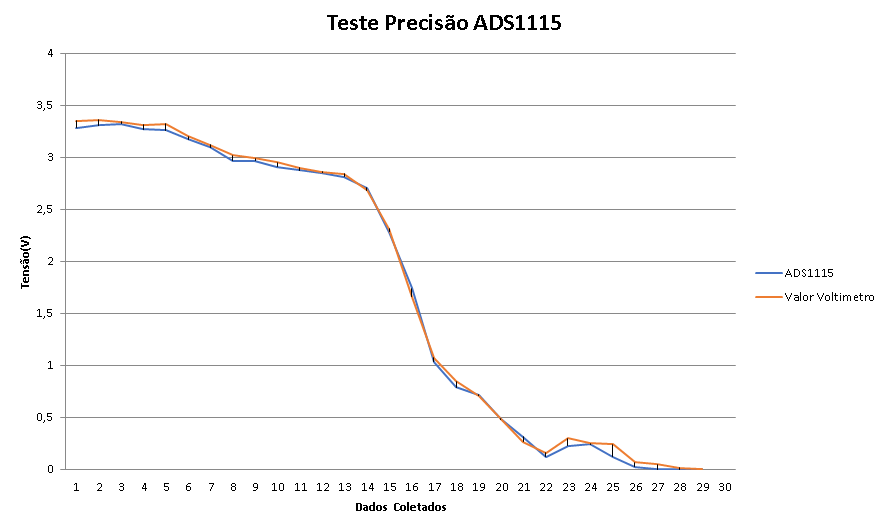
\includegraphics[scale=1.0]{imagens/Precisao}
	\caption{30 diferentes valores de tensão e comparação entre o sensor e um multímetro comercial. Fonte: Elaborado pelo Autor. 	}
	\label{fig:Precisao}
\end{figure}
\FloatBarrier

Considerando a necessidade de testes do traçador I-V, foi utilizado lâmpada halógena como fonte de irradiância. Desta forma foi possível viabilizar os testes mesmo em dias com pouca irradiância e foi possível manter uma irradiância sempre constante durante os testes, figura~\ref{fig:LampII}.  

\FloatBarrier
\begin{figure}[!htbp]
	\centering
	%scale redimensiona a figura.
	%1.5 = 150% do tamanho original
	%1 = 100% do tamanho original
	%0.20 = 20% do tamanho original
	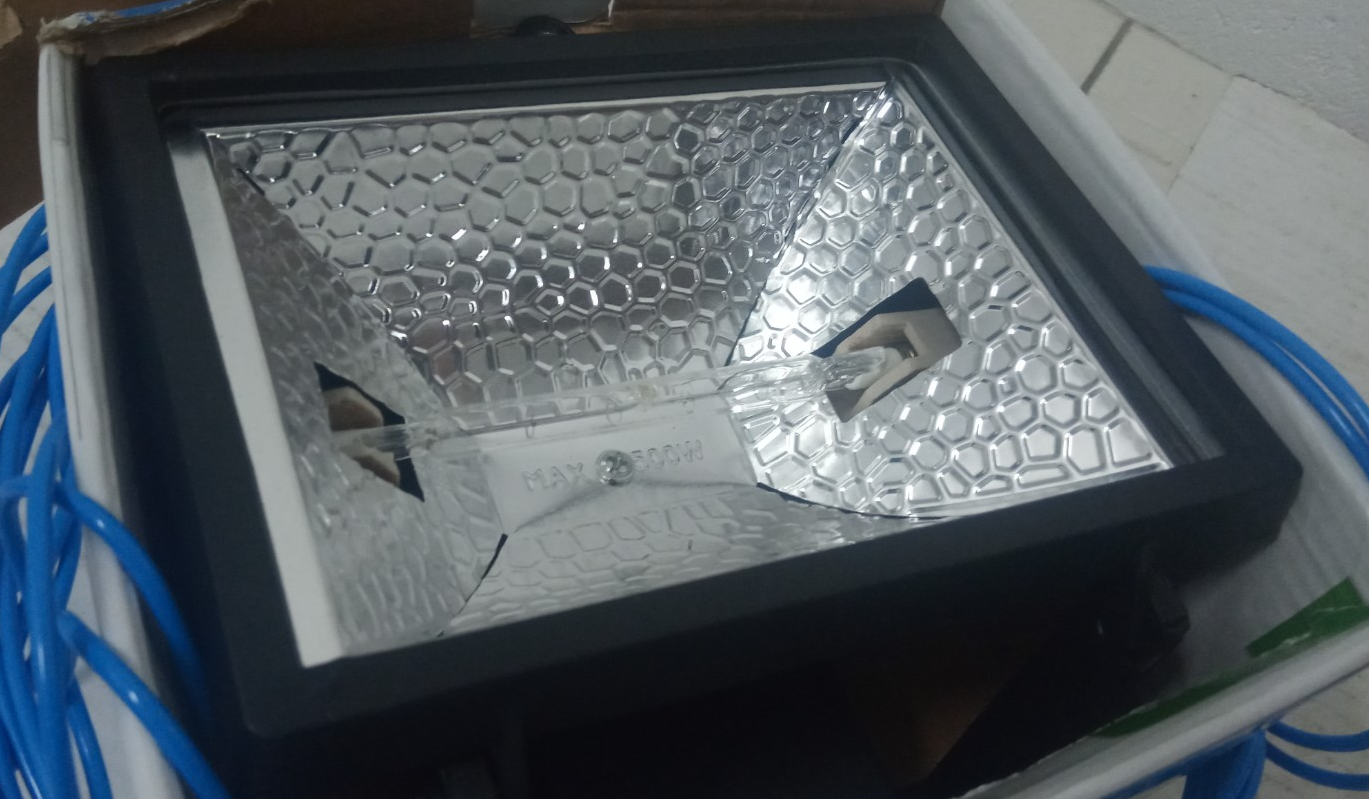
\includegraphics[scale=0.3]{imagens/LampII.png}
	\caption{Lâmpada utilizada. Fonte: Elaborado pelo Autor. 	}
	\label{fig:LampII}
\end{figure}
\FloatBarrier

\subsection{Comportamento do Protótipo}

Para mostrar o estágio de execução da medição, foram instalados LEDs que apresentam em qual parte do processo de aquisição de dados o traçador se encontra, e um LED para sinalização de erros durante a aquisição de dados, sendo suas cores:

\begin{itemize}
	\item Amarelo;
	\item Branco;
	\item Verde 1;
	\item Verde 2;
	\item Vermelho.
\end{itemize}

Foram utilizadas diferentes combinações de LEDs para sinalizar as diferentes etapas, assim como  reproduzido na tabela~\ref{tab:LEDS}.

\FloatBarrier
\begin{table}[!htbp]
	\centering
	\caption{Combinação dos LEDs de sinalização}
	\begin{tabular}{ c | c }
		\hline
		\textbf{Combinações de Cores} & \textbf{Função}                                   \\ \hline
		Vermelho                      & Erro durante a coleta                             \\ \hline
		Amarelo,Verde1                & Aguardando habilitação pelo usuário para a coleta \\ \hline
		Verde2                        & Coleta de dados habilitada                        \\ \hline
		Branco                        & Coletando de dados                                \\ \hline
		Branco,Verde1,Vermelho        & Finalização da coleta                             \\ \hline
	\end{tabular}
	\\ \vspace{0.2cm}
	\textbf{Fonte:} Elaborada pelo autor
	\label{tab:LEDS}
\end{table}
\FloatBarrier

Ao se utilizar da interface através dos LEDs foi possível tornar a coleta de dados mais dinâmica, de maneira a facilitar o uso do usuário e a verificação das etapas e o possível aparecimento de erros.

Tendo a interface pronta, e o circuito montado pronto para os testes, houve então a primeira verificação. Os primeiros experimentos foram feitos utilizando uma Resistência \textit{Shunt}(RS) de aproximadamente 3 Ohms, o que causou uma grande deformação na curva proveniente dos valores coletados.

Após novos testes com diferentes resistências, foi  possível chegar ao resultado mais próximo do esperado ao se utilizar dois resistores de 1 Ohm em paralelo. Houve também a necessidade de alterar alguns pontos da programação tendo a finalidade de se obter mais pontos e garantir uma melhor resolução da curva.




\chapter{Resultados e Discussão}
\label{cap:04}

\title{Resultados Parciais}

Os primeiros circuitos de testes foram construídos em uma Matriz de Contato (\textit{Protoboard}), de modo a facilitar ajustes e adequações de projeto. Para os experimentos foi utilizado uma lâmpada halogena, possibilitando um ambiente controlado para testes, de modo a não depender das condições climáticas ideias para efetuar o experimento. Para alterar a potência de irradiação luminosa expelida pela lâmpada sobre o painel, utilizou-se diferentes distâncias entre a lâmpada e o painel fotovoltaico. Para atestar a alteração da potência irradiada pela lâmpada sobre a superfície do painel, fez-se o uso do solarímetro.

\FloatBarrier
\begin{figure}[!htbp]
	\centering
	%scale redimensiona a figura.
	%1.5 = 150% do tamanho original
	%1 = 100% do tamanho original
	%0.20 = 20% do tamanho original
	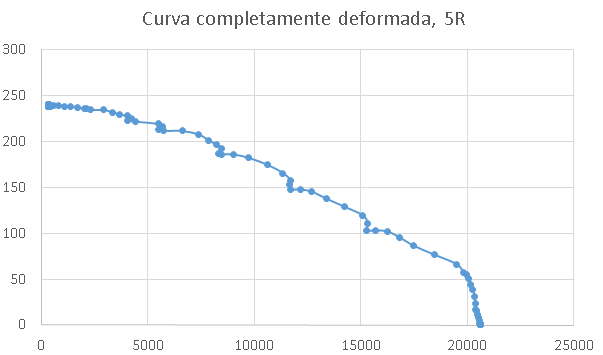
\includegraphics[scale=1]{imagens/CurvaIVdeformadaII}
	\caption{Curva IV deformada devido ao uso de um resistor de 5 Ohms. Fonte: Elaborado pelo Autor. 	}
	\label{fig:CurvaIVdeformadaII}
\end{figure}
\FloatBarrier

%//Acrescentar Imagem de Curvas Morçadas e a foto do circuito na protoboard sem o ADS ou ADC//

Os testes com dos circuitos iniciais não trouxeram os resultados esperados, fazendo com que fosse alterado o projeto. As principais alterações foram a implementação do módulo ADC (ADS1115), a alteração do valor de resistência de carga de 3 para 1 Ohm e a alteração do valor do capacitor de 1000uF para 100uF.

\FloatBarrier
\begin{figure}[!htbp]
	\centering
	%scale redimensiona a figura.
	%1.5 = 150% do tamanho original
	%1 = 100% do tamanho original
	%0.20 = 20% do tamanho original
	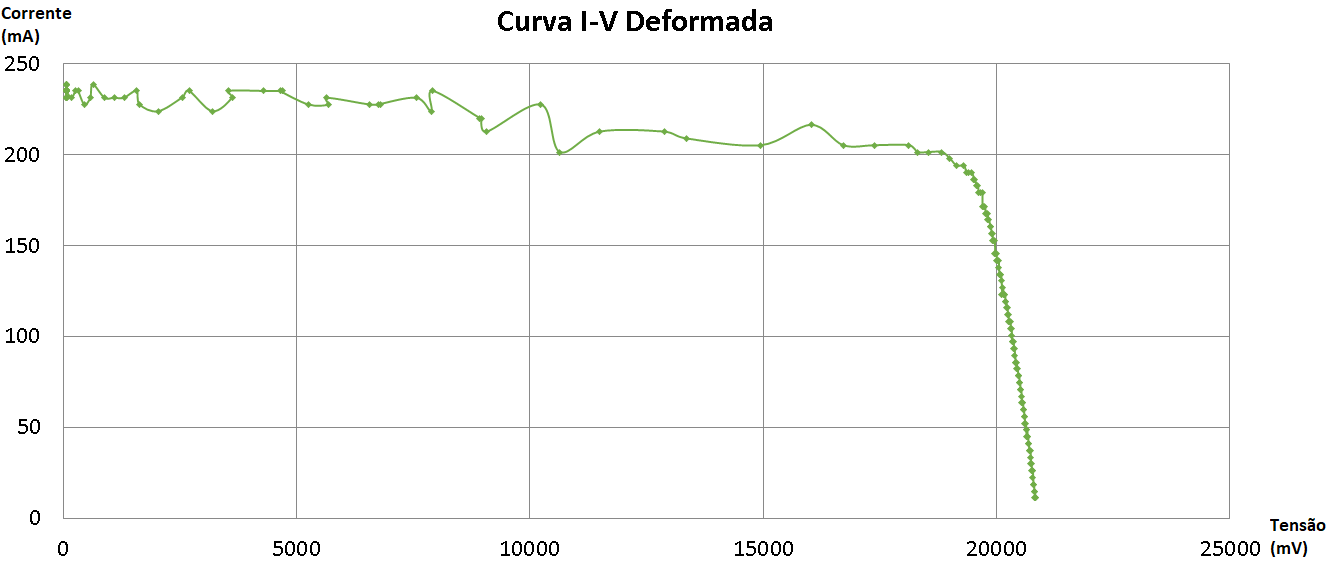
\includegraphics[scale=0.4]{imagens/CurvaIVdeformada}
	\caption{Curva IV deformada devido. Fonte: Elaborado pelo Autor. 	}
	\label{fig:CurvaDeformada}
\end{figure}
\FloatBarrier

%// Acrescentar Imagem de Curvas Morçadas e a foto do circuito na protoboard com o ADS ou ADC//

Com as alterações feitas no circuito, ainda não foi possível obter a curva ideal, de modo que foi necessário efetuar a alteração da programação, configurando diferentes resoluções do pulso de PWM de modo que foi possível traçar curvas com diferentes números de pontos de observação.

\FloatBarrier
\begin{figure}[!htbp]
	\centering
	%scale redimensiona a figura.
	%1.5 = 150% do tamanho original
	%1 = 100% do tamanho original
	%0.20 = 20% do tamanho original
	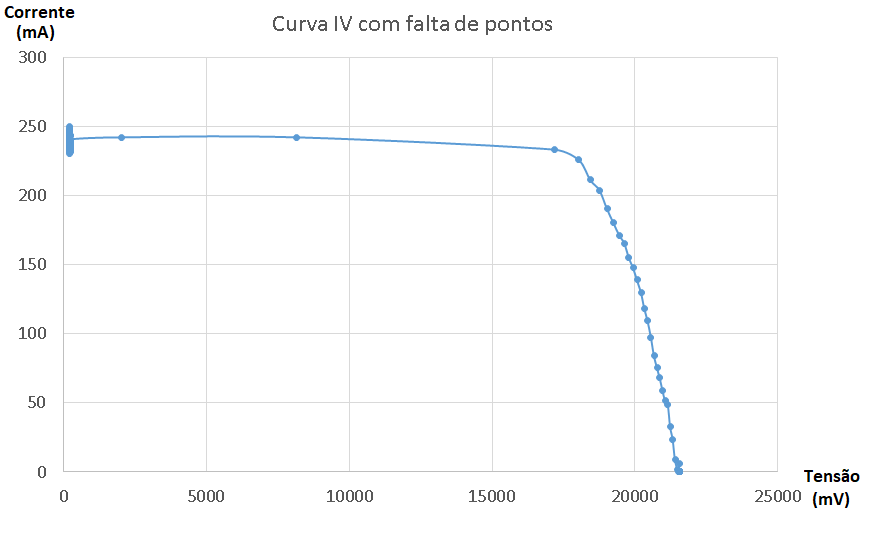
\includegraphics[scale=0.7]{imagens/CurvaIVpoucospontos}
	\caption{Curva IV com poucos pontos. Fonte: Elaborado pelo Autor. 	}
	\label{fig:Curvapoucos}
\end{figure}
\FloatBarrier

%// Acrescentar imagens de Curvas quaaase ideais só que com pouco pontos//.

Após efetuar ajustes no circuito e na programação , foi concluída a fase de teste na \textit{protoboard} obtendo exito na parte experimental. Foi possível traçar a curva I-V ideal do painel fotovoltaico e analisar seu comportamento em diferentes níveis de irradiância solar simulada.
CurvaIVpoucospontos

// Acrescentar fotos do Circuito na protoboard sendo testado (Tirar foto Logo menos), e acrescentar as curvas topzeras)

Resultados Finais:
Após concluir a fase de testes, iniciou-se a fase de confecção do circuito oficial, passando a configuração da \textit{protoboard} para uma placa de circuito impresso.... (Continua nos próximos episódios)  Texto dos resultados.
\chapter{Conclusões}
\label{cap:05}

A maior contribuição deste projeto se dá no processo de criação de um traçador de curvas IV para painéis fotovoltaicos de baixa potência, desde a importância por trás do seu uso para atestar o funcionamento correto, bem como para seu uso em estudos e testes de sombreamento e defeitos o sobre painéis fotovoltaicos. O trabalho também apresentou a possibilidade de ocorrer erros durante o desenvolvimento e teste dos circuitos, desta maneira facilitando o processo de replicação e melhoria do traçador aqui apresentado, garantindo assim o incentivo ao uso e estudo de energia fotovoltaica. Outro aspecto se dá no baixo custo do protótipo, como visto no Anexo~\ref{Anx1}, o qual apresenta o valor total gasto em componentes para replicar o projeto.

A fim de viabilizar o estudo foi utilizado um ambiente de testes estático para o desenvolvimento do traçador utilizando lâmpada halógena de $500$ $W$, esse ambiente permitiu testes contínuos e com variáveis controladas, de maneira a proporcionou a verificação e correção de defeitos pontualmente. O projeto atual não considera problemas como variações de temperatura, irradiância, nuvens e outros aspectos climáticos. Há também a restrição quanto a potência do painel, 25 V e 8 A, devido ao uso dos resistores divisores de tensão para a diminuição da tensão medida pelo conversor AD, a qual é facilmente transposta pelo uso de diferentes valores para o divisor de tensão. Entretanto, há o valor máximo devido ao MOSFET IRF540N, $V_{DSS} = 100$ V e $I_{D} = 33$ A, de acordo com o Datasheet do fabricante.

No que se diz respeito a esses limitadores, é possível a produção de trabalhos futuros com o uso de componentes que permitam painéis de diferentes potências. Há também a possibilidade de testes com painéis com defeitos internos e conjuntos de painéis tendo entre eles defeituosos e plenos. Outra possibilidade está no uso de um traçador utilizando capacitores e uma possível comparação entre a curva do painel por carga eletrônica e a curva do painel por capacitor.

Outros possíveis trabalhos podem ser modelados a partir do uso da lâmpada halógena, com o uso de formas diferentes das utilizadas neste trabalho, posicionada paralelamente em relação ao painel, é possível simular a projeção do sol durante o dia em diferentes horários do dia, além da simulação de diferentes climas, sendo assim adicionado mais variáveis como temperatura externa, temperatura sobre o painel, etc.

Como outra sugestão de possíveis trabalhos se dá na criação de um algoritmo de MPPT, o qual tem como princípio a curva IV do painel fotovoltaico. Ao se utilizar um MPPT é possível garantir que o painel possa gerar sua máxima potência em um dado período de tempo no qual está sendo testado.





%\chapter{Cronograma}
%\label{cap:06}

%Cronograma (para a graduação na qualificação)






% ---------------------------------------------------------------------------------
%                                 ELEMENTOS PÓS-TEXTUAIS
% ---------------------------------------------------------------------------------
\postextual


% ----------------------------------------------------------
% Referências bibliográficas
% ----------------------------------------------------------
\bibliography{referencias}


% ----------------------------------------------------------
% Glossário
% ----------------------------------------------------------
%
% Consulte o manual da classe abntex2 para orientações sobre o glossário.
%
%\glossary


% ----------------------------------------------------------
% Apêndices
% ----------------------------------------------------------
% texto ou documento elaborado pelo autor, a fim de complementar sua argumentação, sem prejuízo da unidade nuclear do trabalho,

% ---
% Inicia os apêndices
% ---
%\apendices
%\partapendices

\begin{apendicesenv}
\partapendices

	% Imprime uma página indicando o início dos apêndices
	\chapter{Circuito Completo}
	\label{Anx1}
		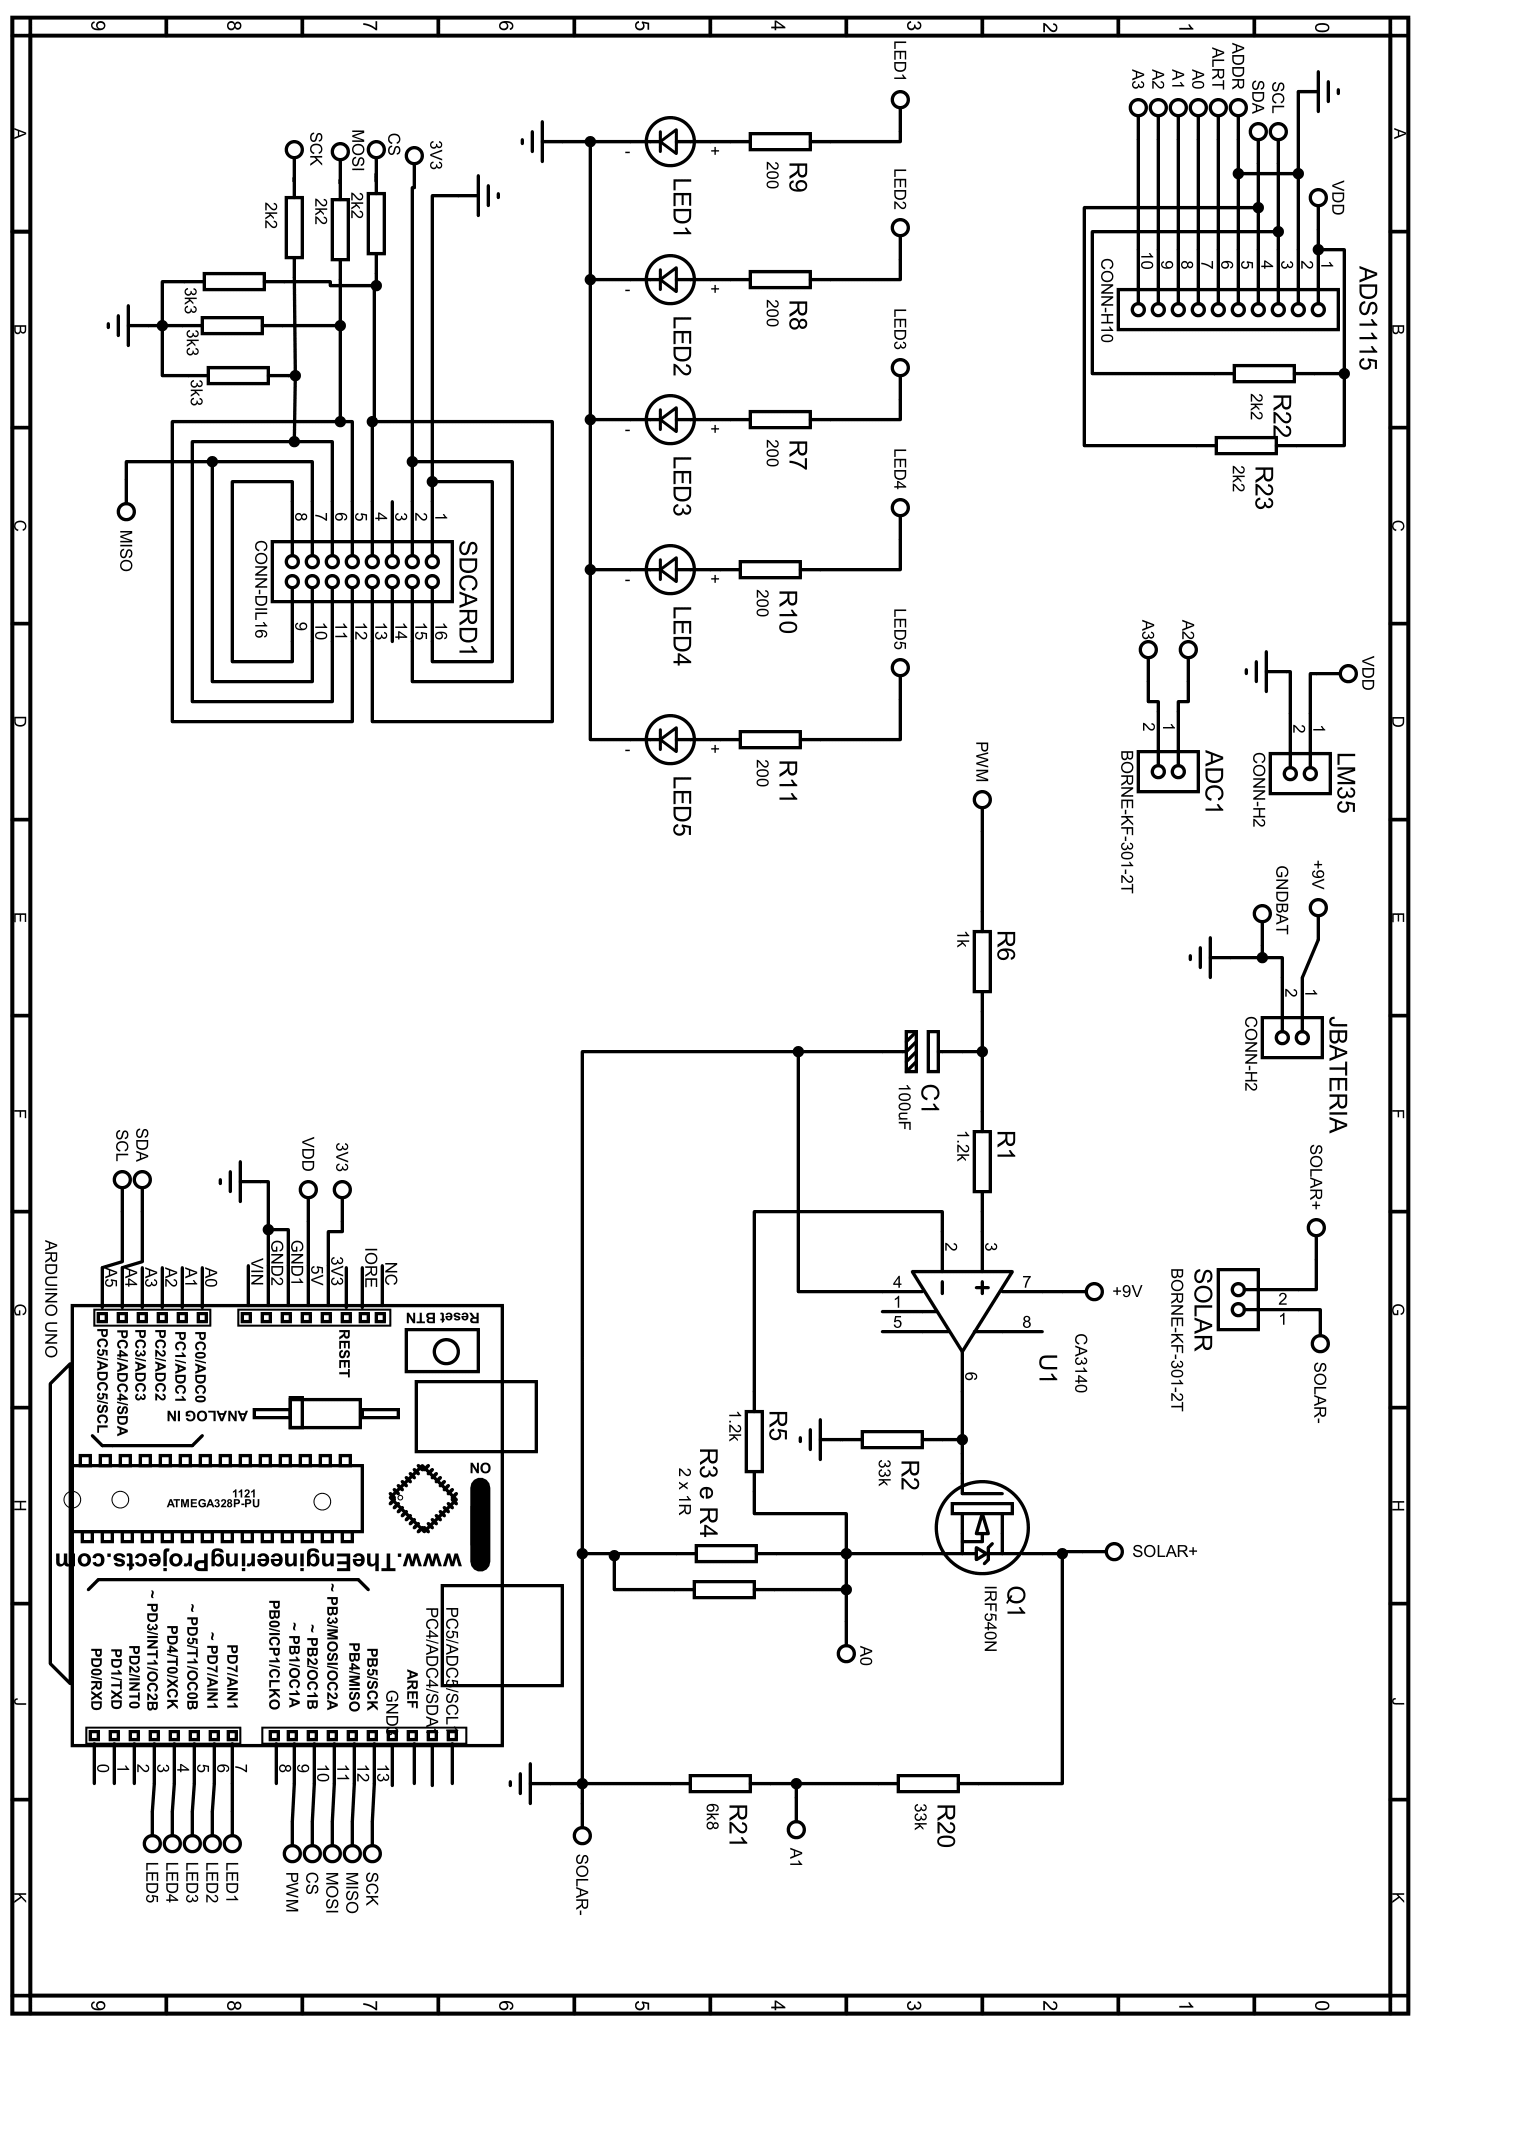
\includegraphics[scale=0.4]{PDFs/AllComponents-rotated-1.png}
	% ----------------------------------------------------------
	\chapter{Título do Apêndice B}
	% ----------------------------------------------------------
	Tabela com o valor gasto para desenvolver um traçador de curva IV.
		\FloatBarrier
		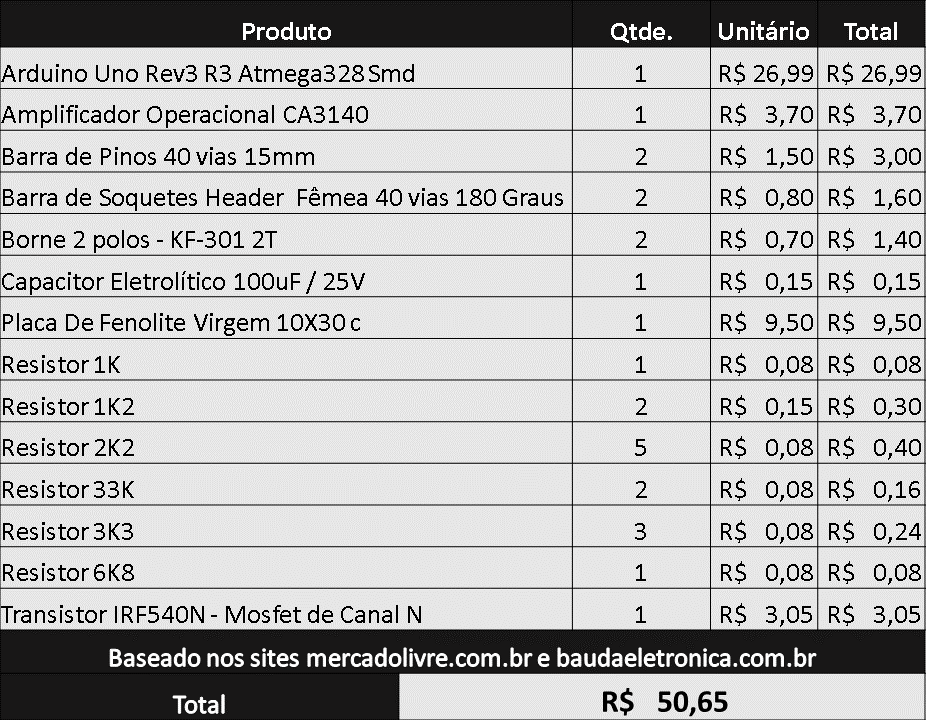
\includegraphics[scale=0.6]{PDFs/values.png}			\FloatBarrier
\end{apendicesenv}
% ---


% ----------------------------------------------------------
% Anexos
% ----------------------------------------------------------
% texto ou documento não elaborado pelo autor, que serve de fundamentação, comprovação e ilustração.

% ---
% Inicia os anexos
% ---
\begin{anexosenv}
	
	% Imprime uma página indicando o início dos anexos
	\partanexos
	
	% ----------------------------------------------------------
	\chapter{Datasheet ADS1115}
	% ----------------------------------------------------------
%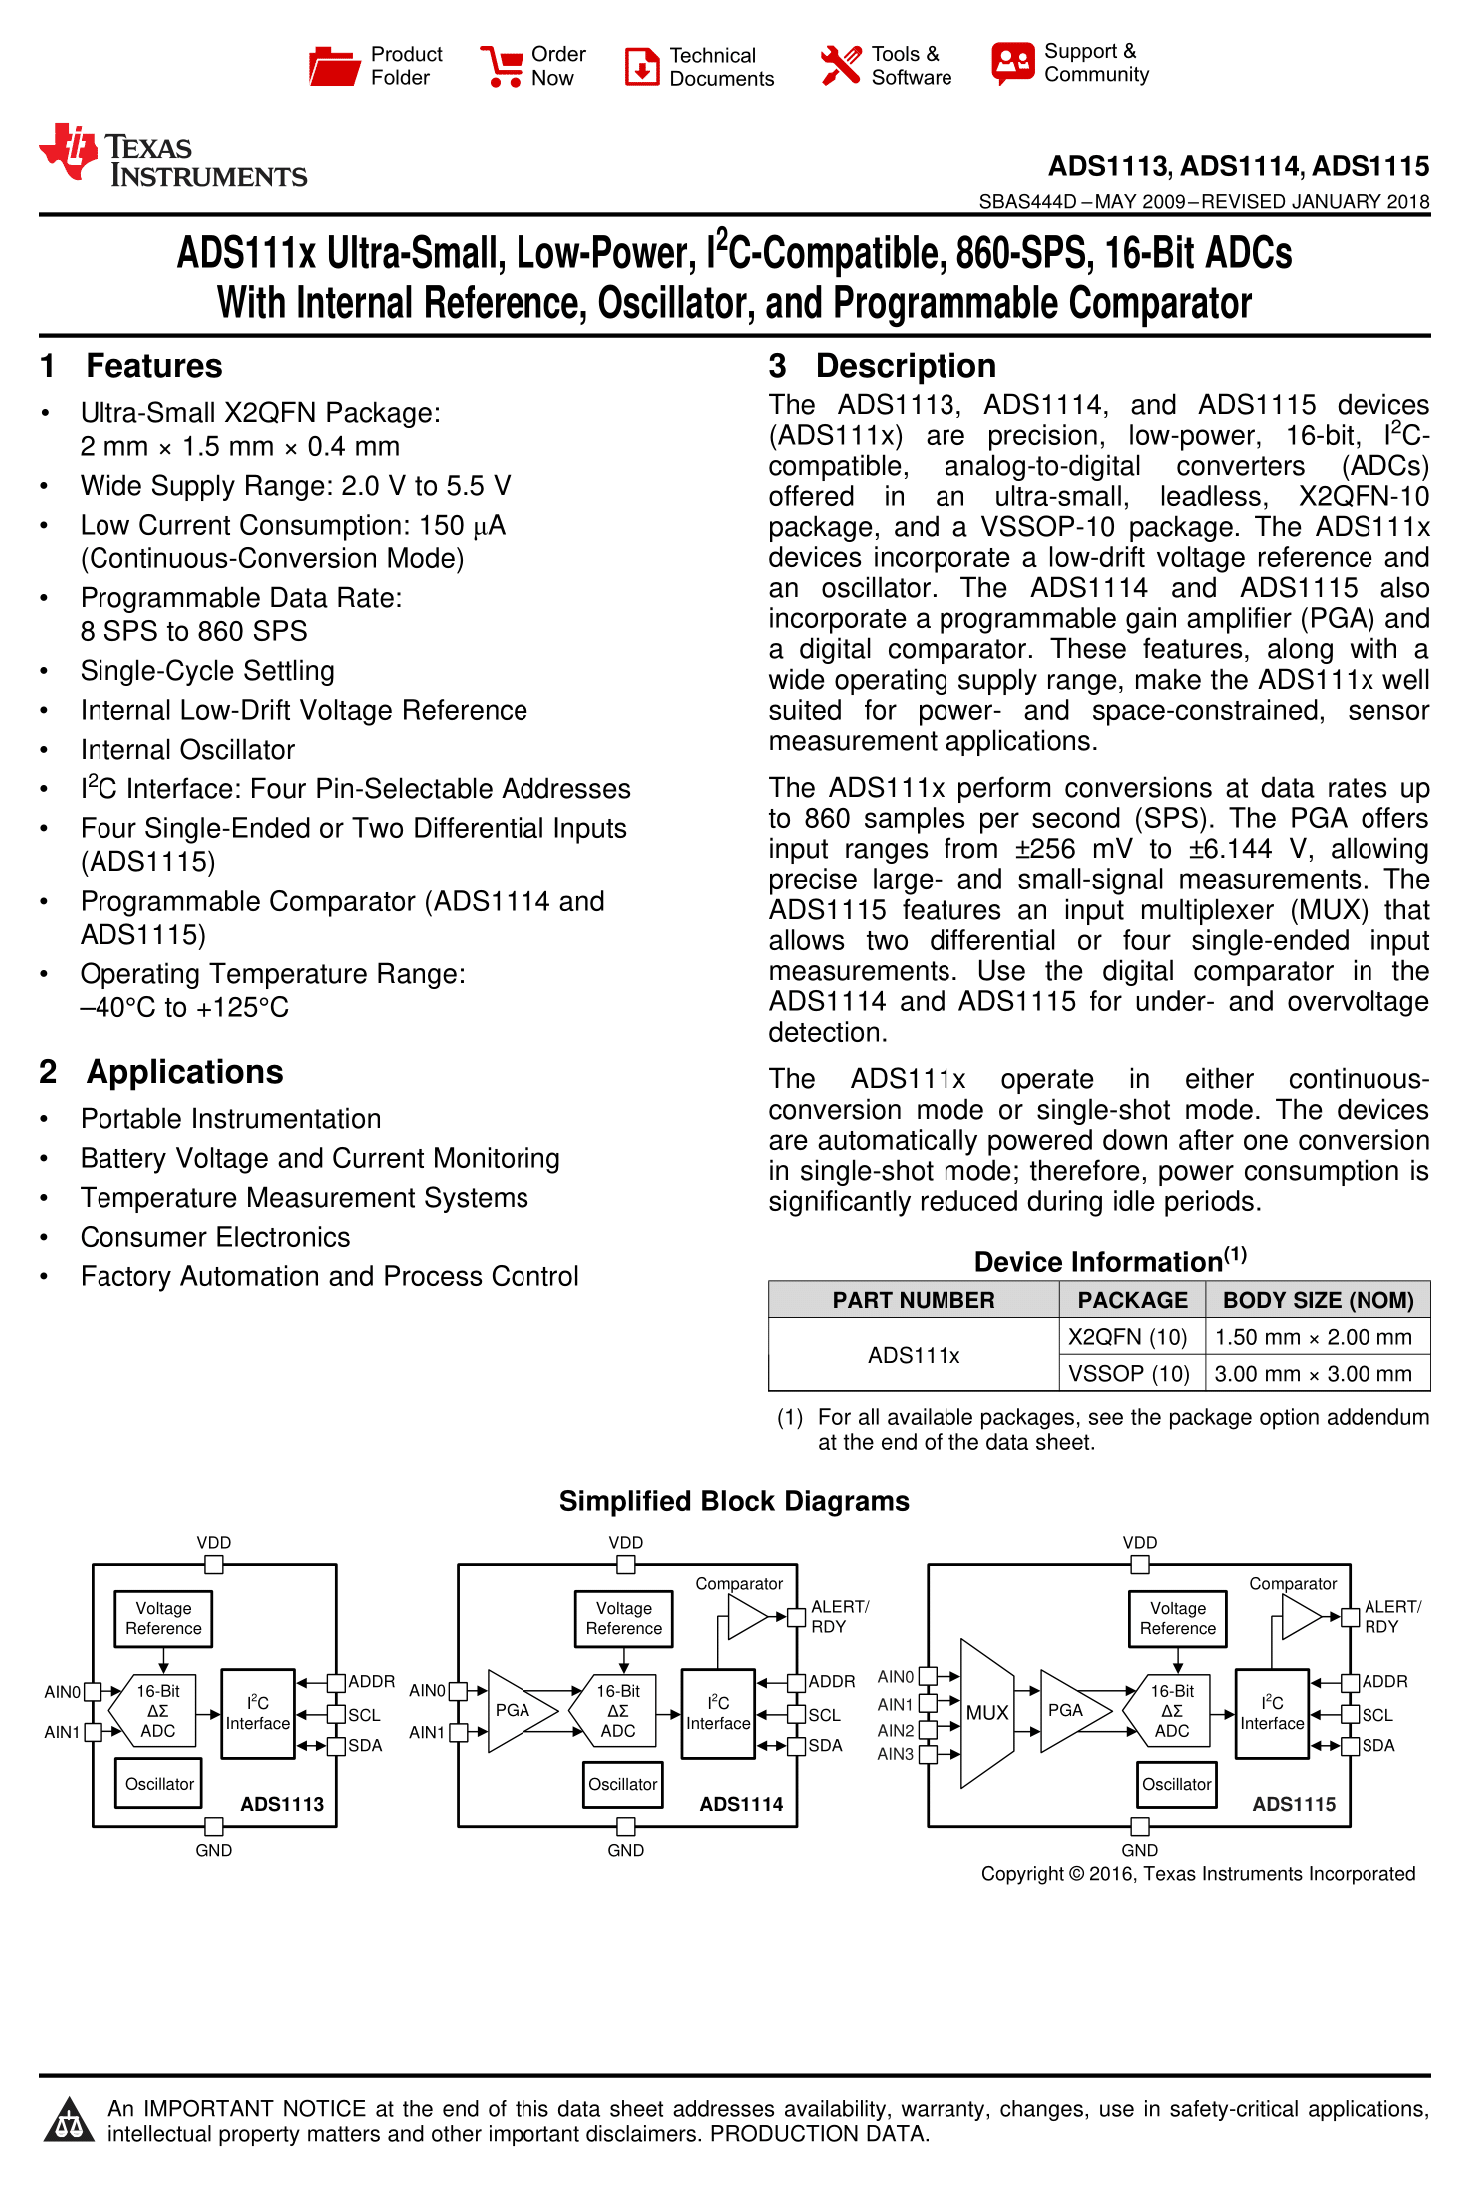
\includepdf[pages=-, scale=0.6]{Anexos/ads1115.pdf}
	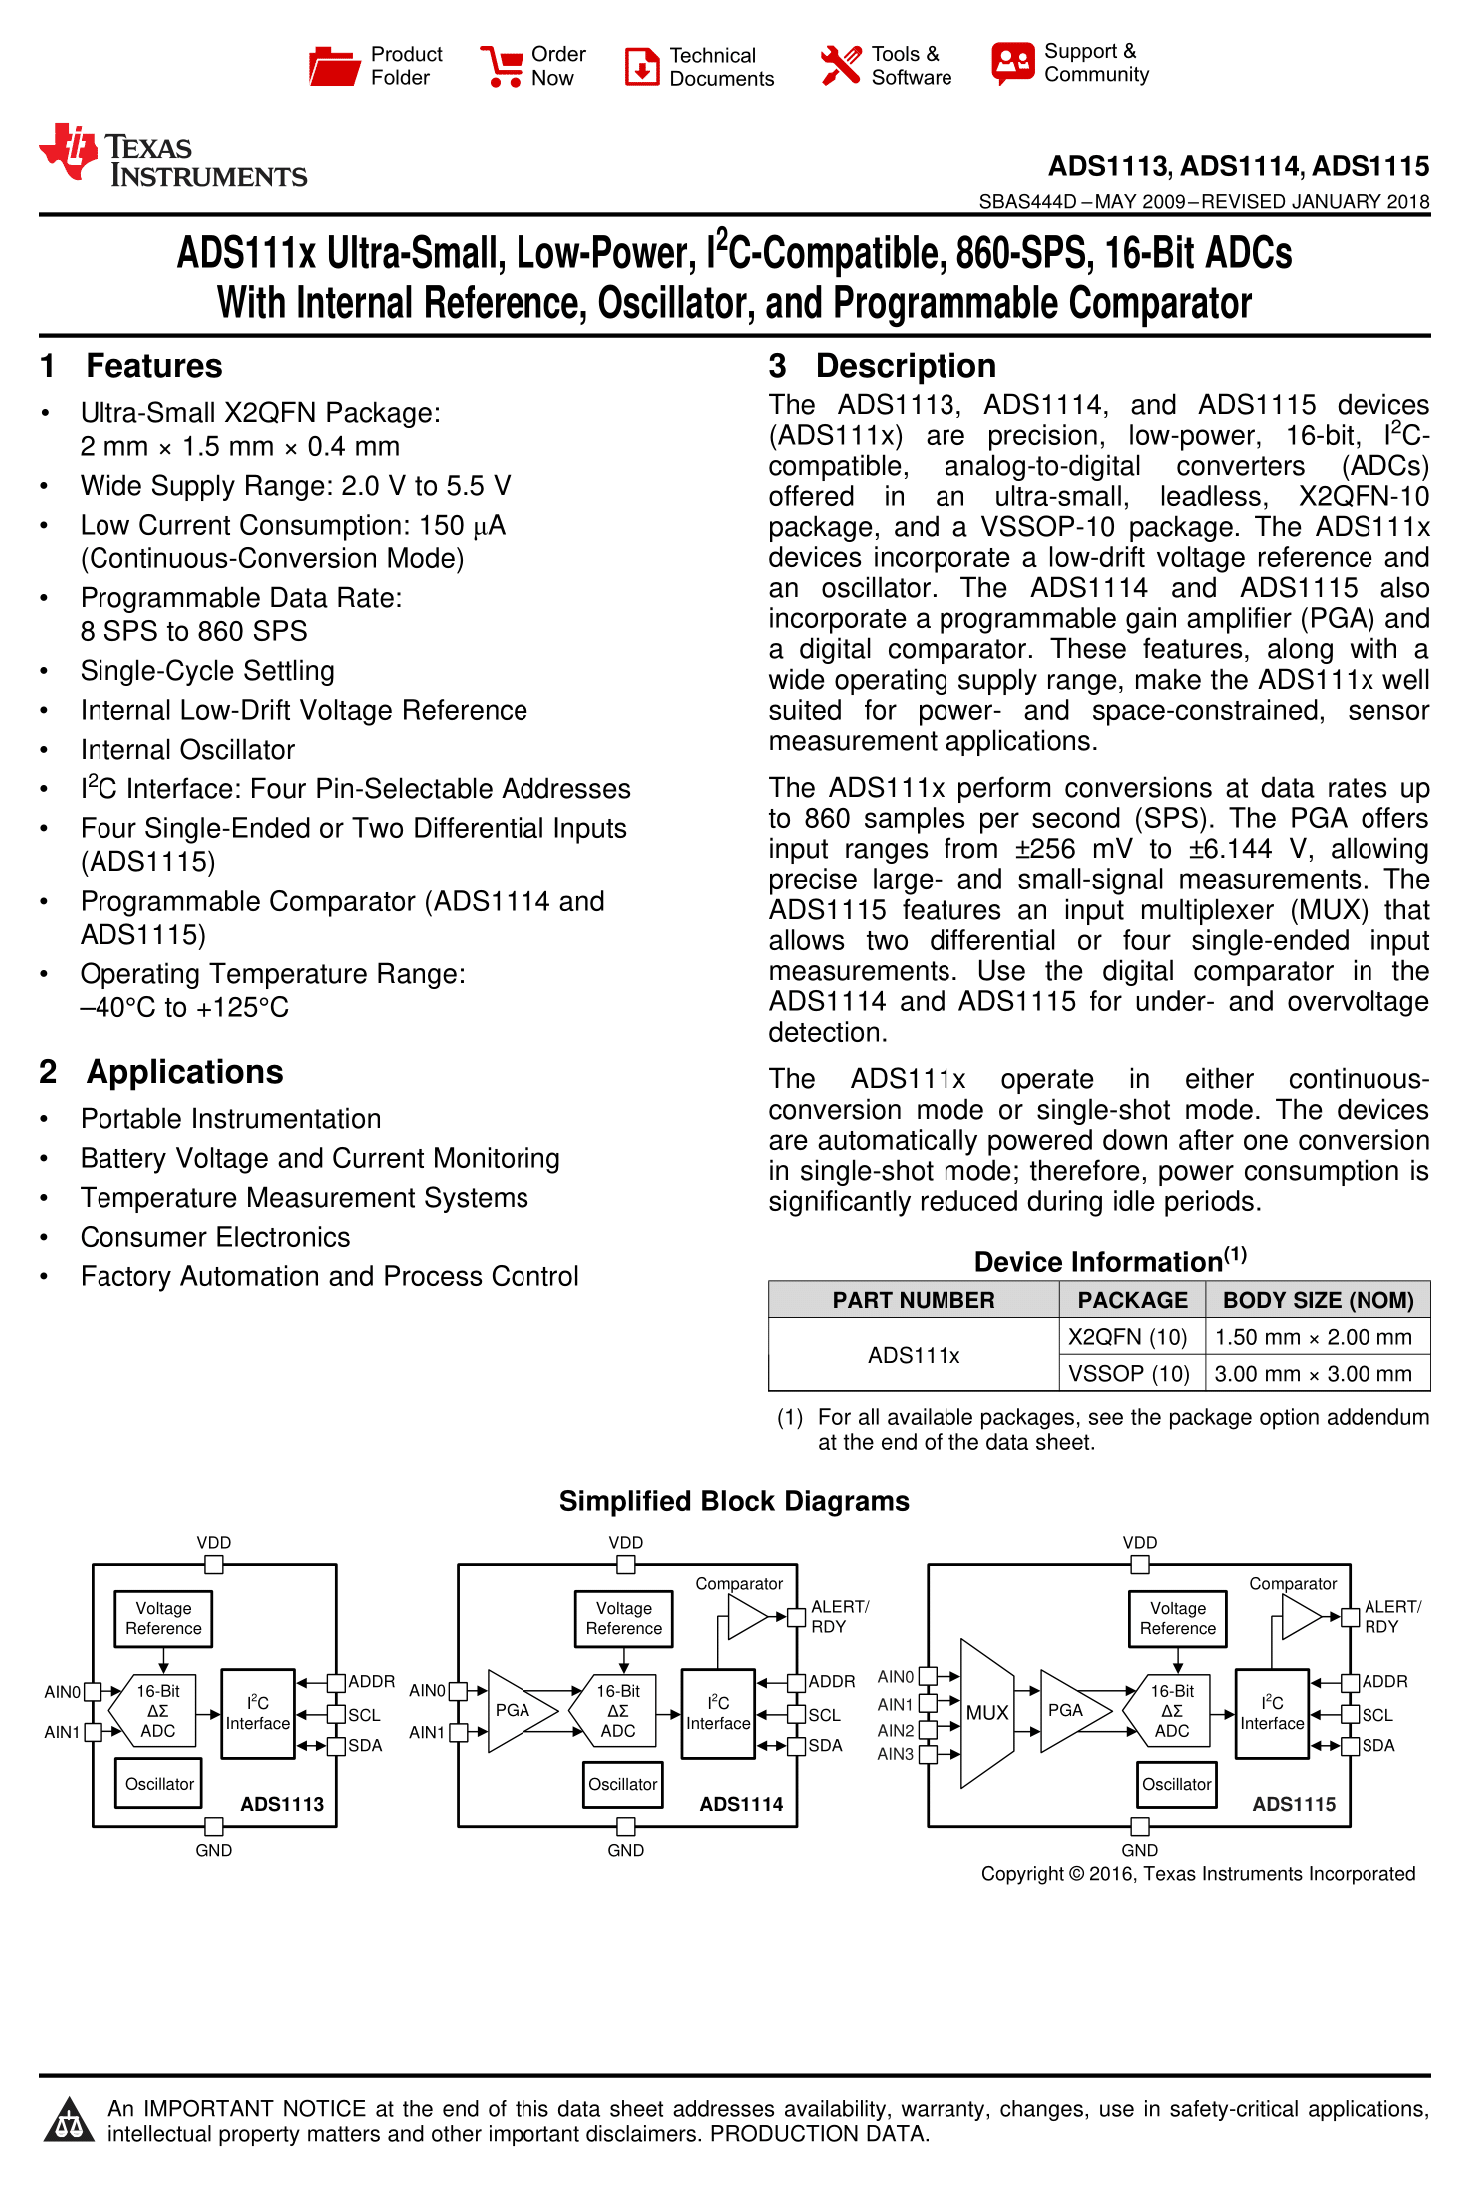
\includegraphics[scale=0.35]{Anexos/ads1115.png}
	
	\FloatBarrier
	Disponível em:\url{http://www.ti.com/lit/ds/symlink/ads1115.pdf}.
%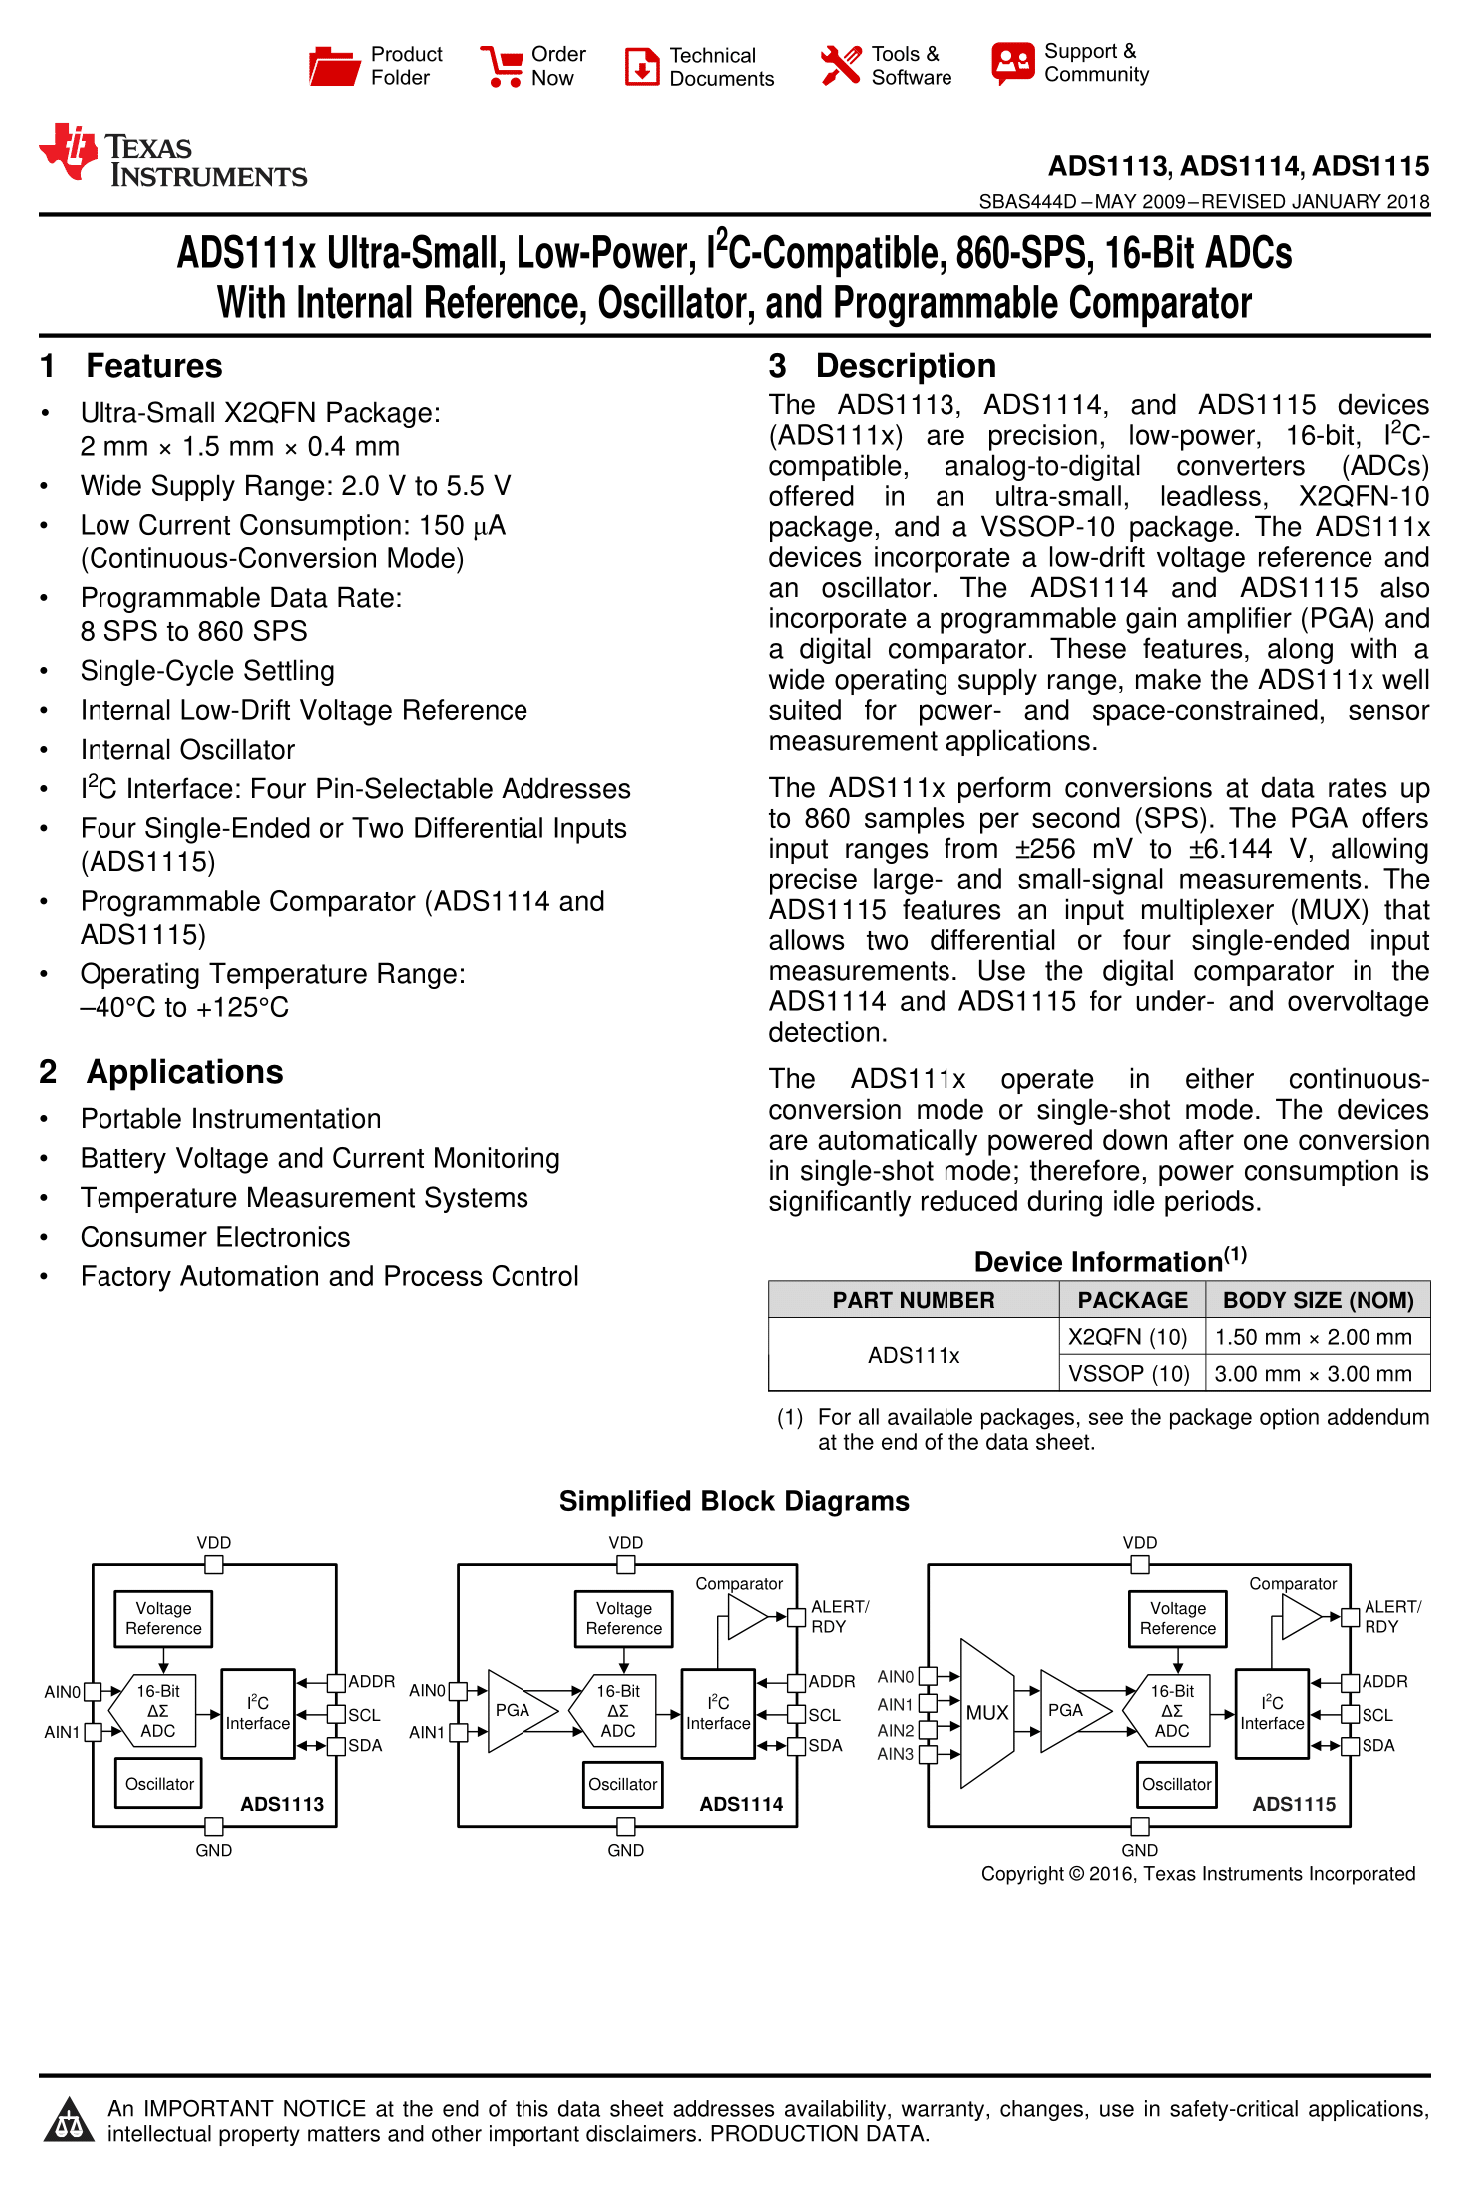
\includepdf[pages=-, scale=0.6, offset=75 -75]{Anexos/ads1115.pdf}

	
	% ----------------------------------------------------------
	\chapter{Título do Anexo B}
	% ----------------------------------------------------------
	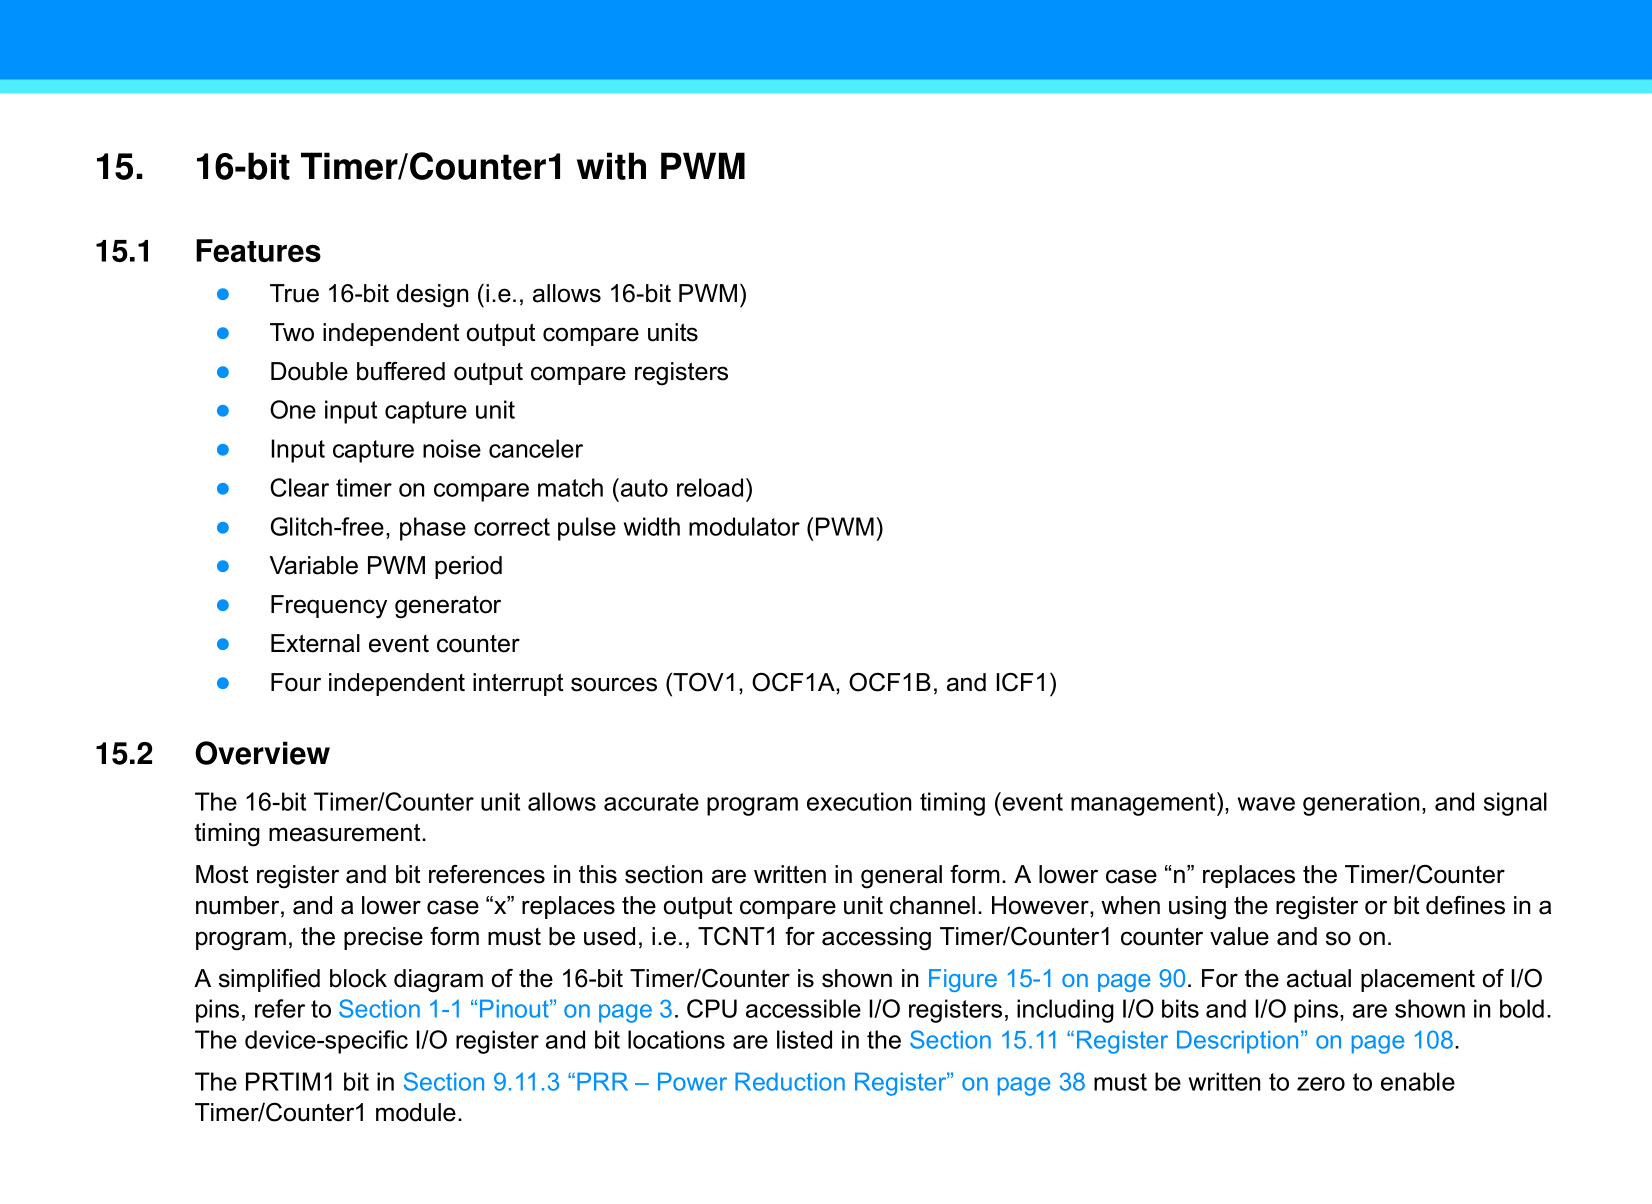
\includegraphics[scale=0.3]{Anexos/Atmel-089.png}
		\FloatBarrier
	Datasheet Atmega328p, Disponível em:\url{http://ww1.microchip.com/downloads/en/DeviceDoc/Atmel-7810-Automotive-Microcontrollers-ATmega328P_Datasheet.pdf}.

\end{anexosenv}


%---------------------------------------------------------------------
% ÍNDICE REMISSIVO
%---------------------------------------------------------------------

%\phantompart

%\printindex


\end{document}
